\usepackage[ngerman, english]{babel}


\title{Attention is All You Need}
\subtitle{overview of the transformer architecture, applications and established improvements}
\author{Felix Karg}


\graphicspath{ {./img/} {../template/} {../template_tex/} } % add further graphics paths here

\newif\iftwocols
% \twocolsfalse
\twocolstrue

% \setbeamertemplate{caption}{\insertcaption}

\usepackage{etex}
\usepackage{graphicx}
\usepackage{color}
\usepackage[export]{adjustbox}
\usepackage{multicol}
\usepackage{pdfpcnotes}
\usepackage{pdfpages}
% \usepackage[dvipsnames]{xcolor}


\usepackage[outputdir={\detokenize{out/main_handout}}]{minted}
\usemintedstyle{pastie}


\usetheme[numbering=counter, progressbar=frametitle, subsectionpage=progressbar]{metropolis}


\date{\today}
% \date{12. Juli 2019}


\institute{Institute for Theoretical Informatics: \newline Artificial Intelligence for Materials Science}
% \titlegraphic{\vspace{4cm} \hspace{7cm} \includegraphics[height=2cm]{Logo_INST}}
\titlegraphic{\vspace{5cm} \hspace{6cm} 
\includegraphics[height=2cm]{AiMat_logo_blue_transparent_rdax_168x76}}

% attempt to reduce space between tableofcontent items in e.g. sectionpage or agenda
\makeatletter
\patchcmd{\beamer@sectionintoc}
  {\vfill}
  {\vskip0\itemsep}
  {}
  {}
\pretocmd{\beamer@sectionintoc}   {\vskip0\itemsep}{}{}
\patchcmd{\beamer@sectionintoc}{\vskip1.5em}{\vskip0.5em}{}{} % <- this one finally works.
\makeatother

% \usepackage{changepage}

% \setbeamertemplate{bibliography item}[text]% {\insertbiblabel}
\addtobeamertemplate{bibliography item}{}{\insertbiblabel}
% \addtobeamertemplate{bibliography item}{\def \bibitemnum {\insertbiblabel}}{}
% \addtobeamertemplate{bibliography entry author}{\insertbiblabel}{}
% \setbeamerfont{bibliography item}{size=\normalsize}
\setbeamercovered{dynamic}

% \AtBeginSection[]
% {
% \begin{frame}[c, plain]
%   \begin{minipage}{22em}
%     \usebeamercolor[fg]{section title}
%     \usebeamerfont{section title}
%
%     % \insertsectionhead\\[-1ex]
%     \iftwocols
%     \begin{multicols}{2}
%     \tableofcontents[currentsection, hideallsubsections]
%     \end{multicols}
%     \else
%     \tableofcontents[currentsection, hideallsubsections]
%     \fi
%
%     % \usebeamertemplate*{progress bar in section page}
%   \end{minipage}
% \end{frame}
% }
% sadly, this does not at all compile and throws weird errors

% from: https://tex.stackexchange.com/questions/365231/enclose-a-custom-quote-environment-in-quotes-from-csquotes
\usepackage[style=british]{csquotes}

\def\signed #1{{\leavevmode\unskip\nobreak\hfil\penalty50\hskip1em
  \hbox{}\nobreak\hfill #1%
  \parfillskip=0pt \finalhyphendemerits=0 \endgraf}}

\newsavebox\mybox
\newenvironment{aquote}[1]
  {\savebox\mybox{#1}\begin{quote}\openautoquote\hspace*{-.7ex}}
  {\unskip\closeautoquote\vspace*{1mm}\signed{\usebox\mybox}\end{quote}}


\iftwocols
\AtBeginSection[]
{
\begin{frame}[c, plain]
  \begin{minipage}{22em}
    \usebeamercolor[fg]{section title}
    \usebeamerfont{section title}
    % \insertsectionhead\\[-1ex]
    % \usebeamertemplate*{progress bar in section page} % progress bar
    \begin{multicols}{2}
    \tableofcontents[currentsection, hideallsubsections]
    \end{multicols}
  \end{minipage}
\end{frame}
}
\else

\AtBeginSection[]
{
\begin{frame}[c, plain]
  \begin{minipage}{22em}
    \usebeamercolor[fg]{section title}
    \usebeamerfont{section title}
    % \insertsectionhead\\[-1ex]
    \tableofcontents[currentsection, hideallsubsections]
    % \usebeamertemplate*{progress bar in section page}
  \end{minipage}
\end{frame}
}
\fi

\AtBeginSubsection[]
{
\begin{frame}[c,plain]
  \begin{minipage}{22em}
    \raggedright
    \usebeamercolor[fg]{section title}
    \usebeamerfont{section title}
    \insertsectionhead\\[-1ex]

    \usebeamertemplate*{progress bar in section page}
    \par
    \ifx\insertsubsectionhead\@empty\else%
      \usebeamercolor[fg]{subsection title}%
      \usebeamerfont{subsection title}%
      \vspace{0.5cm}
      \tableofcontents[sectionstyle=hide/hide,subsectionstyle=show/shaded/hide]
    \fi
  \end{minipage}
\end{frame}
}


%%%%%%%%%%%%%%%%%%%%%%%%%%%%%%%%%%%%%%%%%%%%%%%%%%%%%%%%%%%%%%%%%%%%%%%%%%%%%%%%%%%%%%%%%%%%%%%%%%%
% Newcommand definitions
% - code[1]
% - backupbegin
% - backupend
% - mailto[1]
% - todo[1]
% Environments:
% - codeboxed[1]


\newcommand{\code}[1]{
    \begin{center}
    \setlength{\fboxrule}{1pt}
    \setlength{\fboxsep}{8pt}
        {\fbox{\parbox{0.81\textwidth}{#1}}}
   \end{center}
}

\newenvironment{codeboxed}[1]
        {\begin{minipage}{\linewidth}\begin{center}#1\\[1ex]\begin{tabular}{|p{\textwidth}|}\hline}
        {\\\hline\end{tabular}\end{center}\end{minipage}}


\newcommand{\backupbegin}{
   \newcounter{finalframe}
   \setcounter{finalframe}{\value{framenumber}}
}

\newcommand{\backupend}{
   \setcounter{framenumber}{\value{finalframe}}
}


\newcommand{\mailto}[1]{
    \href{mailto:#1}{#1}
}

\newcommand{\todo}[1]{
    {\Large\color{red}{(TODO: #1)}}
}

% \definecolor{green1}{RGB}{38, 69, 37} % #264525
\definecolor{green1}{RGB}{72, 129, 69} % #488145
% \definecolor{blue1}{RGB}{7, 43, 94} % #072b5e
\definecolor{blue1}{RGB}{14, 82, 179} % #0e52b3
% \definecolor{violet1}{RGB}{58, 38, 68} % #3a2644
\definecolor{violet1}{RGB}{108, 72, 126} % #6c487e
% \definecolor{orang1}{RGB}{, , 0} % #663400
\definecolor{orang1}{RGB}{193, 98, 0} % #c16200

\newcommand{\gray}[1]{
    \textcolor[gray]{0.65}{#1}
}

\newcommand{\green}[1]{
    \textcolor{green1}{#1}
}
\newcommand{\blue}[1]{
    \textcolor{blue1}{#1}
}
\newcommand{\vio}[1]{
    \textcolor{violet1}{#1}
}
\newcommand{\orang}[1]{
    \textcolor{orang1}{#1}
}



%%%%%%%%%%%%%%%%%%%%%%%%%%%%%%%%%%%%%%%%%%%%%%%%%%%%%%%%%%%%%%%%%%%%%%%%%%%%%%%%%%%%%%%%%%%%%%%%%%%
% begin document

\begin{document}
\addtocounter{framenumber}{1}
\maketitle


%%%%%%%%%%%%%%%%%%%%%%%%%%%%%%%%%%%%%%%%%%%%%%%%%%%%%%%%%%%%%%%%%%%%%%%%%%%%%%%%%%%%%%%%%%%%%%%%%%%
% Agenda

\iftwocols

\begin{frame}[c,plain]% {Agenda}
    \begin{minipage}{22em}
    \usebeamerfont{section title}
    \usebeamercolor[fg]{section title}
    % \usebeamertemplate*{progress bar in section page} % progress bar
    \begin{multicols}{2}
    \tableofcontents[hideallsubsections]
%   \tableofcontents[]
    \end{multicols}
    \end{minipage}
\end{frame}

\else

\begin{frame}[c,plain]% {Agenda}
    \begin{minipage}{22em}
    \usebeamerfont{section title}
    \usebeamercolor[fg]{section title}
    \tableofcontents[hideallsubsections]
%   \tableofcontents[]
    \end{minipage}
\end{frame}
\fi




\newif\ifonline
\onlinefalse
% \onlinefalse
% usage:
% \ifonline
%   <true text>
% \else % <- optional
%   <false text>
% \fi

%%%%%%%%%%%%%%%%%%%%%%%%%%%%%%%%%%%%%%%%%%%%%%%%%%BEGINNING%%%%%%%%%%%%%%%%%%%%%%%%%%%%%%%%%%%%%%%%

\section{Overview}
\begin{frame}[c]{Plan}
    Individual Parts:
    \begin{itemize}[<+(1)->]
        \item Normal FeedForward MLP
        \item Embedding: Input
        \item Embedding: Location
        \item Basics of Attention (before transformer)
        \item Attention is All You Need \cite{vaswani_attention_2017}
        \item Linear Attention: FastFormer \cite{wu_fastformer_2021} / Flash Attention \cite{hua_transformer_2022}

        \item (fun:) One Model to Learn Them All \cite{kaiser_one_2017}
        \item Distillation / Quantization \cite{polino_model_2018}
    \end{itemize}
\end{frame}


\section{Background}
\subsection{Multi-Layer Perceptron}
\begin{frame}[c]{Multi-Layer Perceptron}
    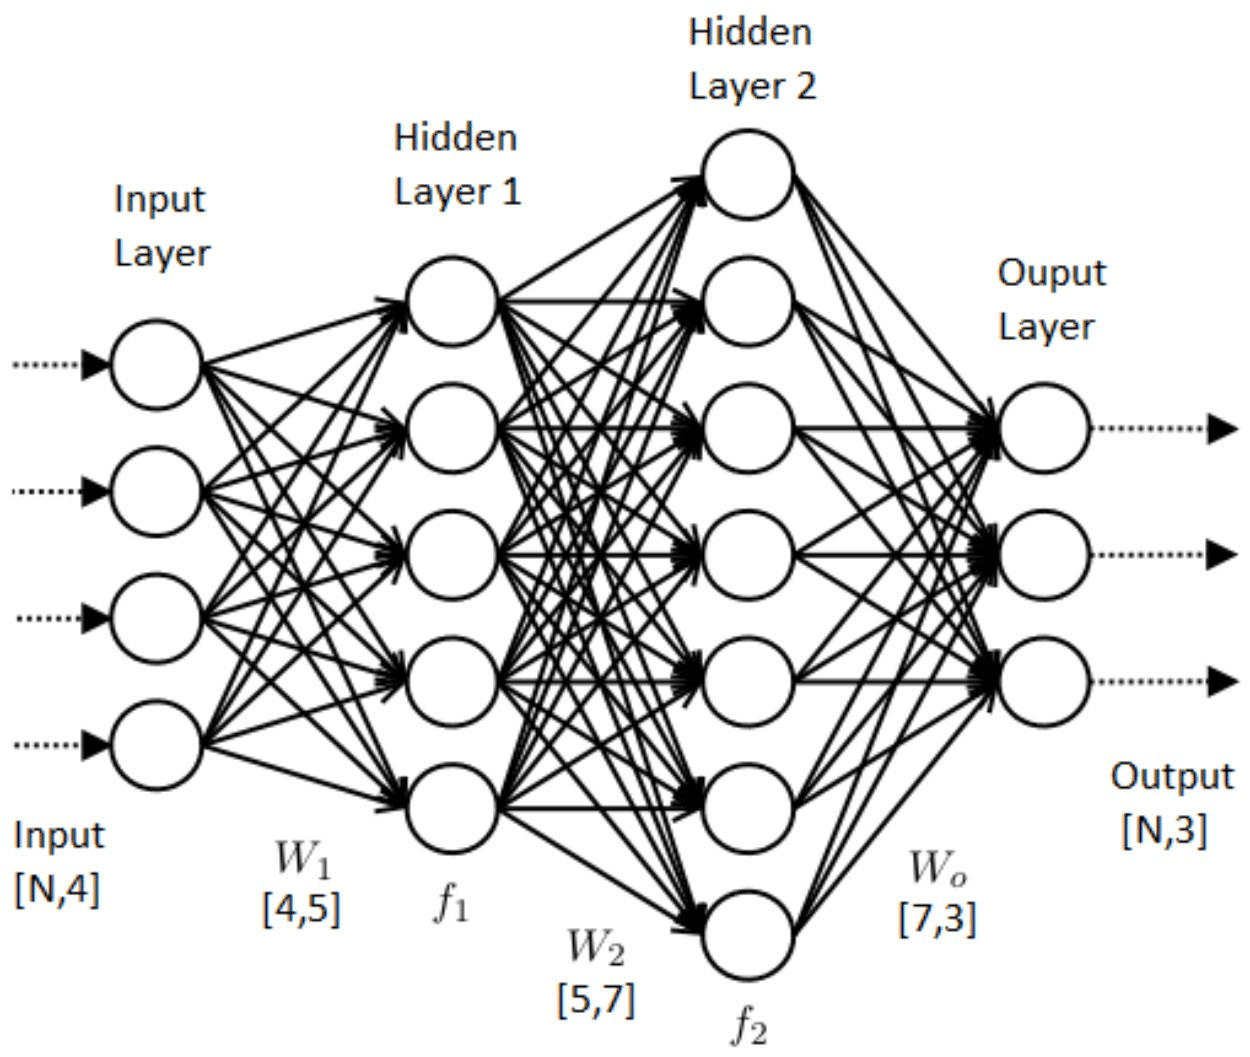
\includegraphics[height=0.85\textheight]{dense_1} \\
    \normalsize
    \gray{Image Source: Public Domain}
    \pnote{
    Classic Dense FF \\
    has some arbitrary nonlinear activation function
    }
\end{frame}

\subsection{Activation Functions}
\begin{frame}[c]{Common Activation Functions}
    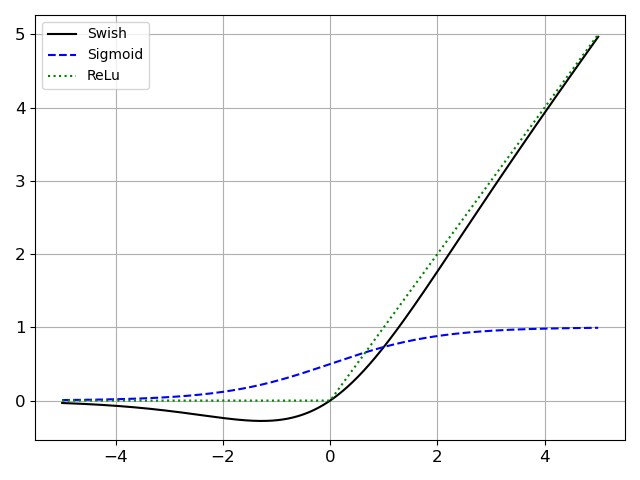
\includegraphics[height=0.75\textheight]{sigmoid_swish_relu} \\
    $swish(x) := x * sigmoid(x)$ \\
    \gray{Image Source: \cite{chen_deep_2021}} \hspace{1cm}
    SwiGLU introduced by \cite{shazeer_glu_2020}
    \pnote{
        GLU = Gated Linear Unit, sigmoid is one too \\
        basically vectorization of activation function
    }
\end{frame}

\subsection{Missing Connections}
\begin{frame}[c]{Dropout I}
    \large
    \textbf{Problem:} neural network training results in highly specialized feature adaptations (overfitting) \\
    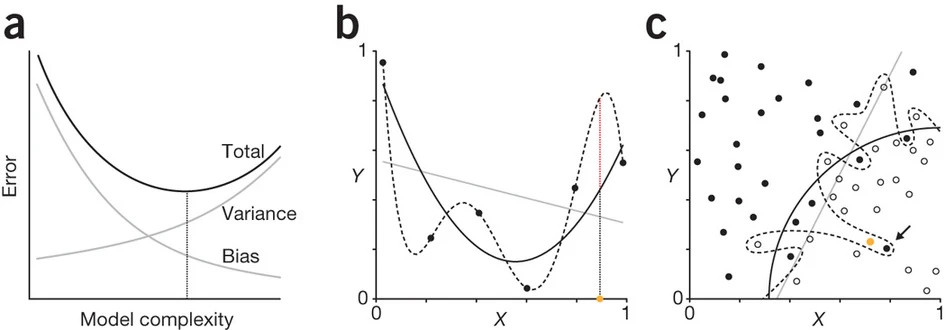
\includegraphics[width=\textwidth]{overfitting} \\
    \normalsize
    \gray{Image Source: \cite{lever_points_2016}}
    % "Complex co-adaptations can be trained to work well on a training set, but on novel test data they are far more likely to fail than multiple simpler co-adaptations that achieve the same thing." \cite{srivastava_dropout_2014}
    \pnote{
        benefits: generalization of features across multiple nodes, \\
        which makes them less pronet to overfitting \\
        \\
        For some reason, not used by a lot of modern LLMs
    }
\end{frame}

\begin{frame}[c]{Dropout II}
    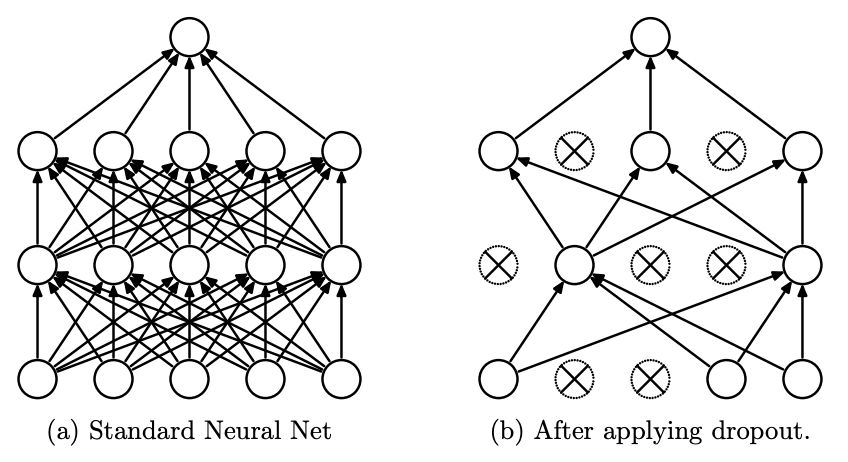
\includegraphics[width=\textwidth]{dropout} \\
    \gray{Image Source: \cite{srivastava_dropout_2014}}
    \pnote{
        Dropout arbitrarily removes neurons during training \\
        => no reliance on individual features \\
        \\
        Effectively results in an ensamble of different \\
        networks, averaging the output during testing. \\
        Powerful method for regularization \\
        \\
        Well-known mechanism for Random Forests
    }
\end{frame}


\subsection{Going Deeper}
\begin{frame}[c]{Residual Connections}
    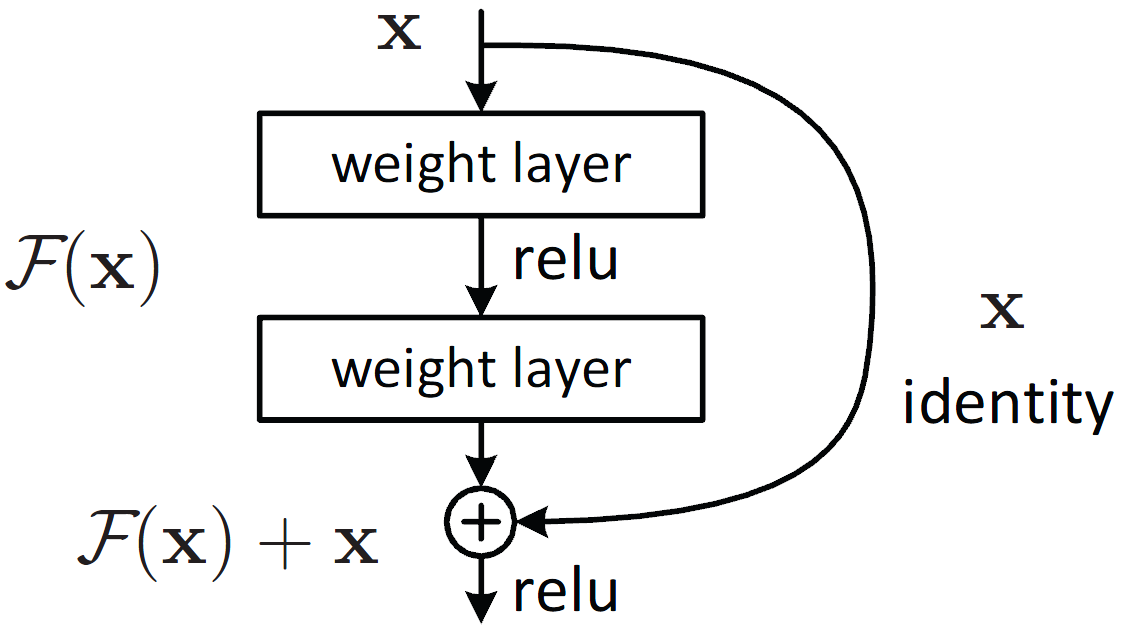
\includegraphics[width=\textwidth]{resnet} \\
    \gray{Image Source: \cite{he_deep_2016}}
    % \large
    % \newline
    % \newline
    % \pause
    % \textbf{Also:} Feature Pyramid Networks \cite{lin_feature_2017} in CV
\end{frame}


\begin{frame}[c]{Perplexity}
    Measure for language modeling capacity
    \todo{build slide}
\end{frame}

\section{Embedding}
\subsection{Overview}
\begin{frame}[c]{Step I: Embedding}
    % trim=l b r t
    \includegraphics[height=0.9\textheight,clip,trim=120 0 120 0]{Transformer_initial_embeddings}
    \raisebox{3em}{\gray{Image Adapted from \cite{vaswani_attention_2017}}}
\end{frame}


\begin{frame}[c]{Definitions}
    \large
    \begin{itemize}[<+(1)->]
        \item    \textbf{Token:} String of arbitrary length
        \item    \textbf{Vocabulary:} List of tokens available to the tokenizer, that can be recognized and generated \\
        \item    \textbf{Tokenizer:} Splitting input text apart using available tokens from the vocabulary \\
        \item    \textbf{Embedding:} Internal high-dimensional representation of given set of tokens (learned) \\
        % \item    \textbf{Mapping:} Individual tokens still need a mapping to an embedding (learned) \\
    \end{itemize}
    \pause
    The Vocabulary / Tokens are commonly learned via Byte Pair
    Encoding (BPE) \cite{shibata_byte_1999}. \\
    \pause
    \small (SOTA library: sentencepiece \cite{kudo_sentencepiece_2018})
    \pnote{
        Tokens usually include the ascii alphabet and other common strings
    }
\end{frame}


\begin{frame}[c]{Overview of Individual Steps}
    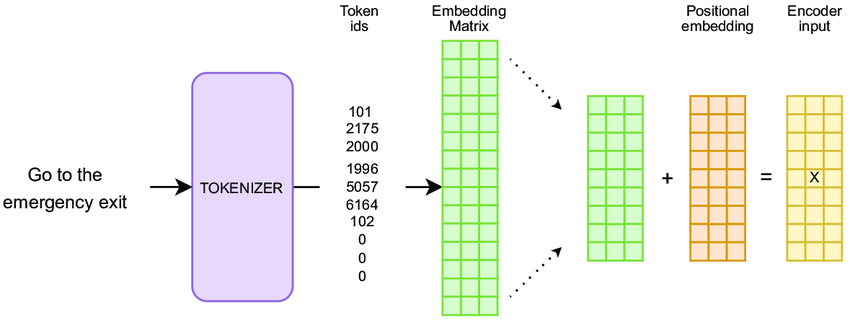
\includegraphics[width=\textwidth]{tokenizer_embedding} \\
    \gray{Image Source: \cite{arici_realworld_2023}} \\
    \large
    Visualization of Encoding pipeline.
\end{frame}

\subsection{Input Embedding}
\begin{frame}[c]{Input Embedding}
    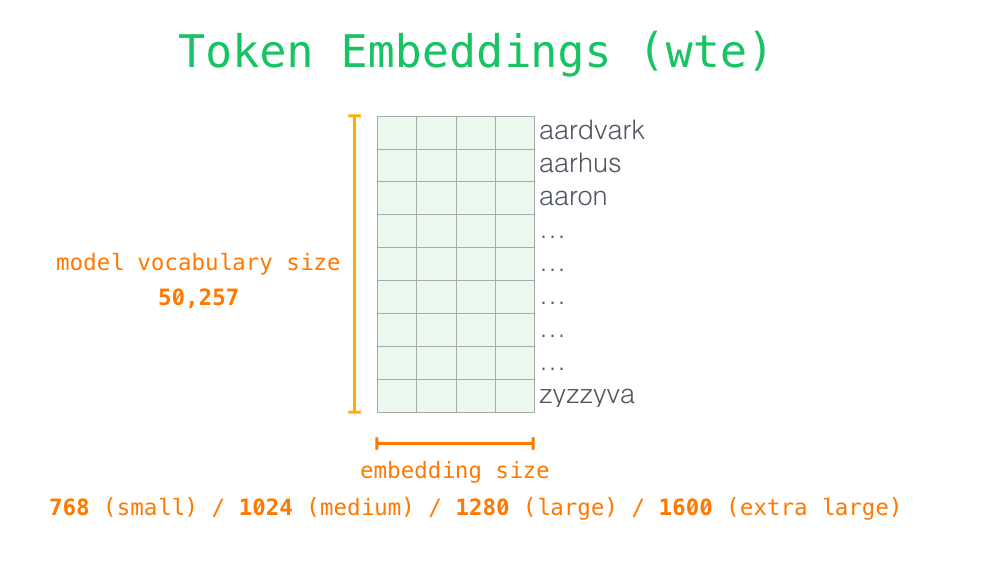
\includegraphics[width=\textwidth]{gpt2-token-embeddings-wte-2} \\
    \gray{Image Source: \cite{alammar_illustrated_2019}} \\
    \large
    Exemplary token to embedding encoding in GPT2.
\end{frame}

\begin{frame}[c]{In Code}
    \inputminted{python}{code/embedding.py}
\end{frame}

\subsection{Positional Encoding}

\begin{frame}[c]{Positional Encoding}
    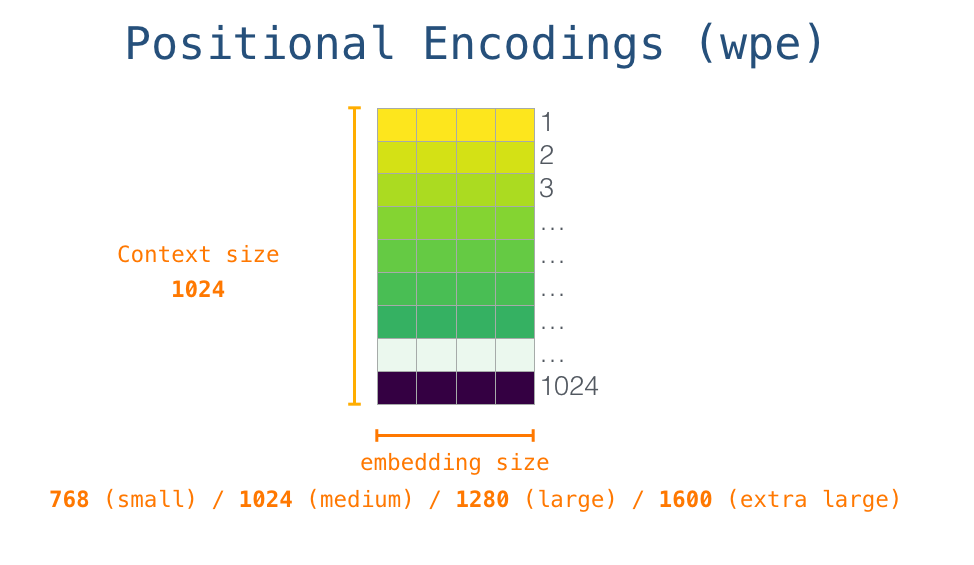
\includegraphics[width=\textwidth]{gpt2-positional-encoding} \\
    \gray{Image Source: \cite{alammar_illustrated_2019}} \\
    \large
    Exemplary positional encoding in GPT2.
\end{frame}

\begin{frame}[c]{Positional Encoding II}
    \large
    \textbf{Visualization} of a sinusoidal position encoding for the first 128 positions in 512 dimensions.
    \newline
    \newline
    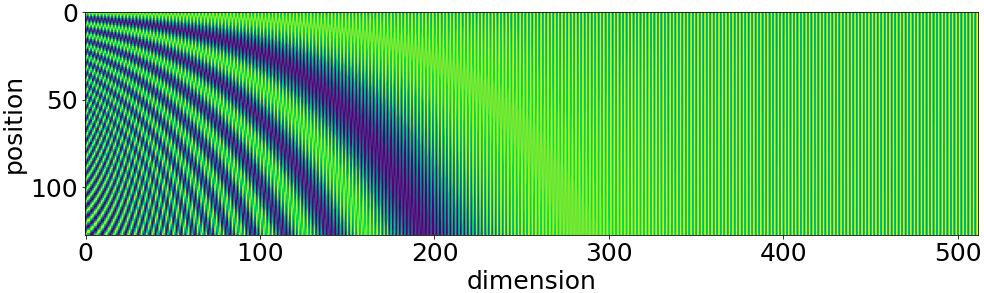
\includegraphics[width=\textwidth]{positional_encoding} \\
    \normalsize
    \gray{Image Source: Public Domain}
\end{frame}

\begin{frame}[c]{RoPE: Rotary Positional Encoding (SOTA)}
    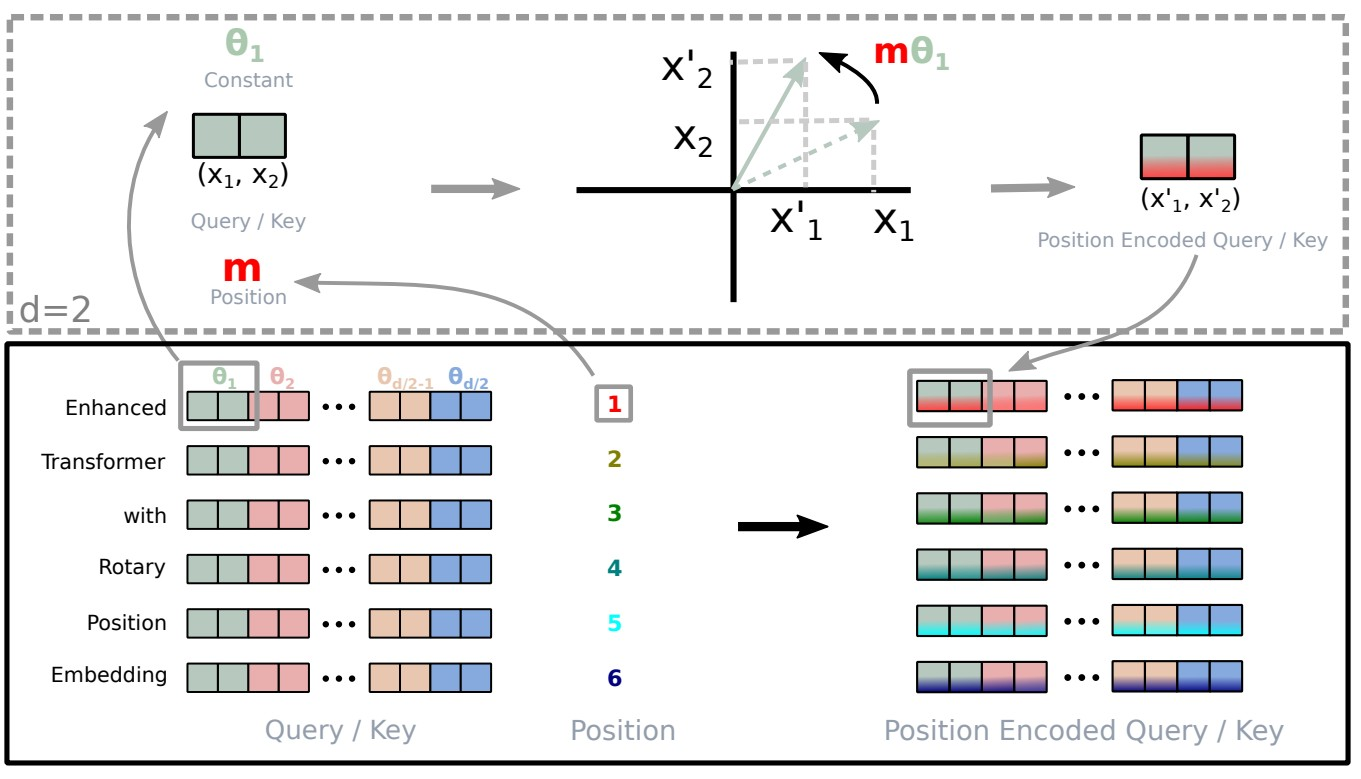
\includegraphics[width=\textwidth]{rope} \\
    \gray{Image Source: \cite{su_roformer_2022}}
    \pnote{
        Used for newer models, e.g. LLaMa or Falcon
    }
\end{frame}


\subsection{Full Input Embedding}
\begin{frame}[c]{Full Input Embedding}
    % trim=left bottom right top, clip
    \includegraphics[width=\textwidth,trim=0 0 0 700,clip]{Transformer_initial_embeddings}
    \gray{Image Adapted from \cite{vaswani_attention_2017}} \\
    \large
    Simple Addition. Works well due to sparse high dimensional spaces.
\end{frame}



\section{Attention}

\begin{frame}[c]{Attention in Transformer}
    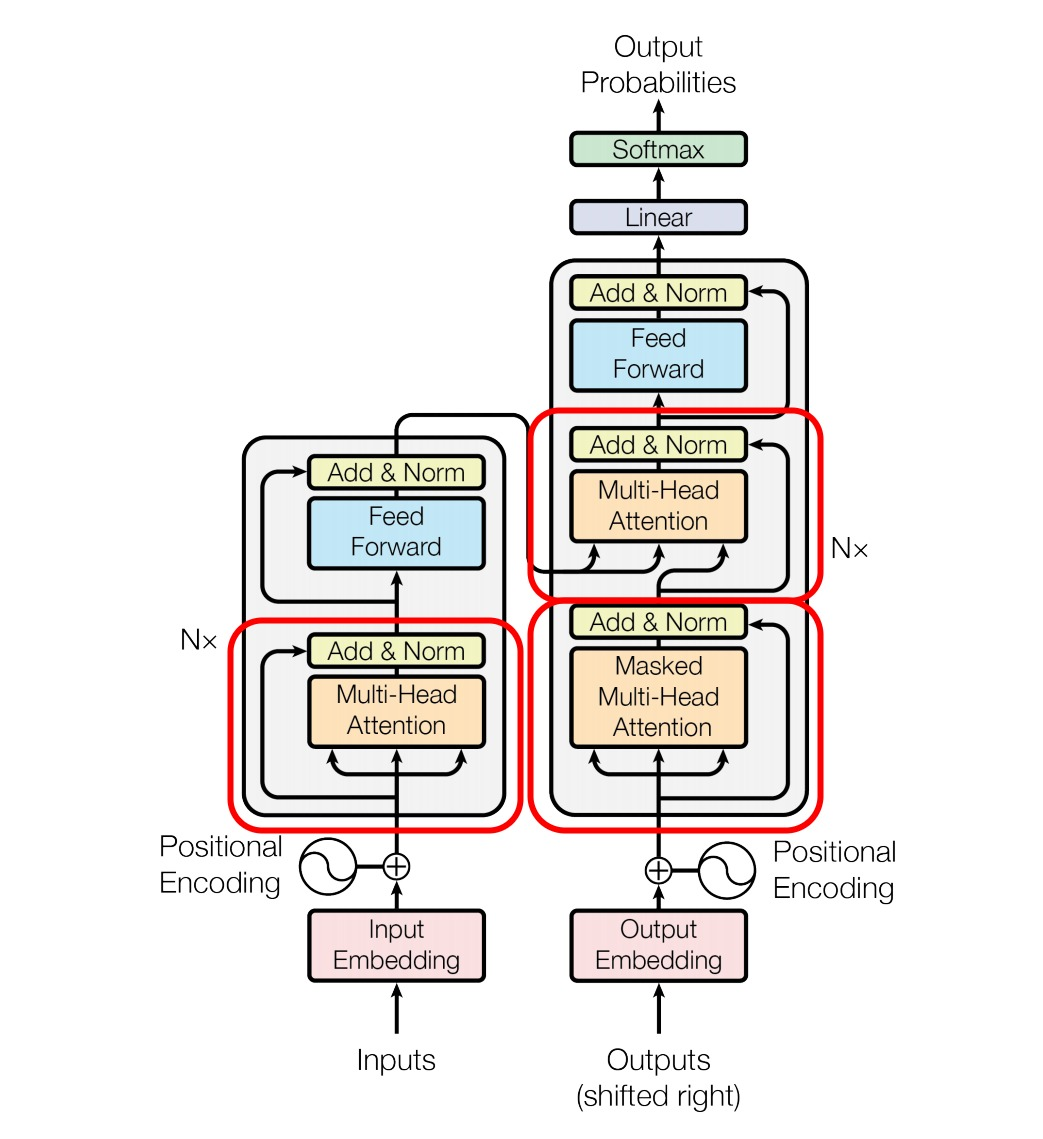
\includegraphics[height=0.9\textheight,clip,trim=120 0 120 0]{transformer_attention}
    Image Adapted from \cite{vaswani_attention_2017}
\end{frame}


\subsection{Basic Attention}

\begin{frame}[c]{Basic Attention}
    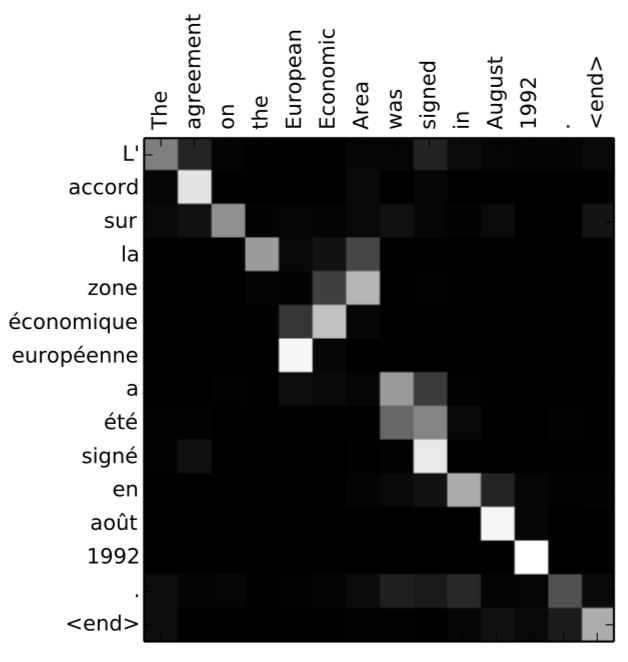
\includegraphics[height=0.85\textheight]{neural-alignment} \\
    Image Source: \cite{bahdanau_neural_2016}
    \pnote{
        Attention existed before the transformer \\
        architecture, but was used in combination \\
        with recurrent neural networks. \\ \\
        As seen here, it focuses on what is learned relevant
    }
\end{frame}

\begin{frame}[c]{Attention Mechanism}
    \large
    $$attention(Q, K, V) = softmax(\frac{QK^T}{\sqrt{d_k}})V$$
    \pause
    where
    $$Q = W_Q\textcolor{blue}{x}, K = W_K\textcolor{blue}{x}, V = W_V\textcolor{blue}{x}, \text{ and } d_k \text{ query-size}$$
    for self-attention \pause and
    $$Q = W_Q\textcolor{blue}{x}, K = W_K\textcolor{red}{y}, V = W_V\textcolor{red}{y}$$
    for encoder-decoder cross-attention
    \pnote{
        d_k is query-size dimension
    }
\end{frame}


\begin{frame}[c]{Scaled Dot-Product Attention}
    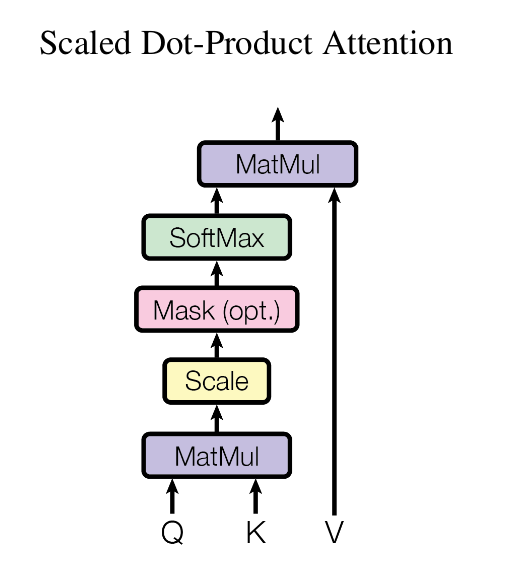
\includegraphics[height=0.9\textheight]{scaled_dot_attention}
    Image Source: \cite{vaswani_attention_2017}
\end{frame}


\subsection{Multi-Head Attention}
\begin{frame}[c]{Multi-Head Attention}
    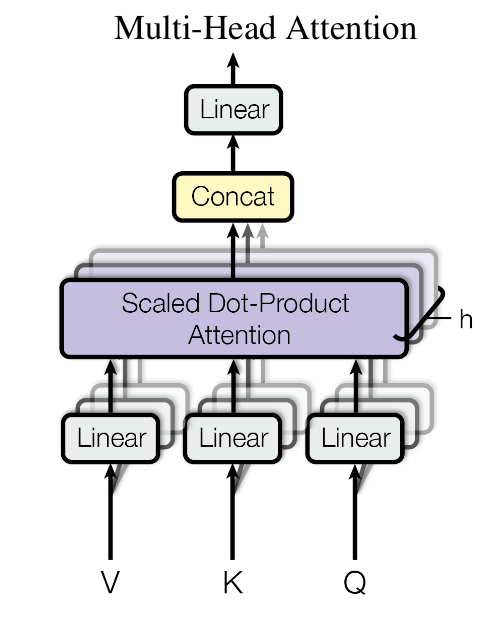
\includegraphics[height=0.9\textheight]{multi_head_attention}
    Image Source: \cite{vaswani_attention_2017}
    \pnote{
        As I understand it, MHA is for splitting the
        embedding space in different partitions, ensuring that each part get's
        at least a certain amount of 'activation'. This can increase
        performance considerably, but effectively it doesn't do
        anything different. Effectively black magic, but seems to
        work.
    }
\end{frame}

\subsection{Masked Attention}
\begin{frame}[c]{Masked Attention}
    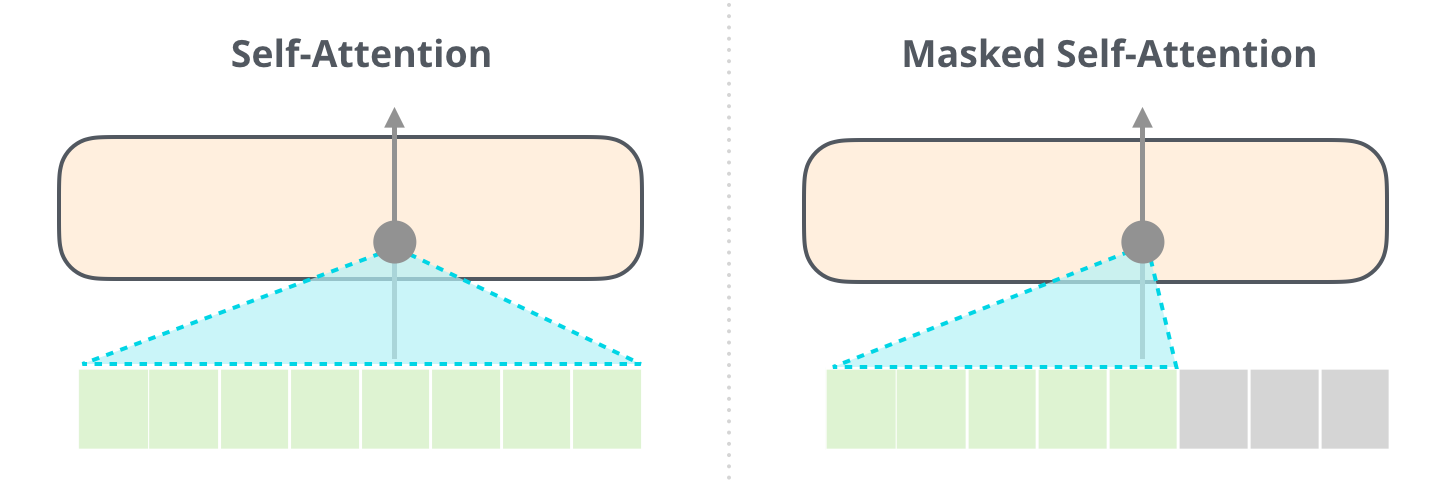
\includegraphics[width=\textwidth]{masked-self-attention} \\
    Image Source: \cite{alammar_illustrated_2019}
\end{frame}


\section{Transformer}

\subsection{Output}
\begin{frame}[c]{Output}
    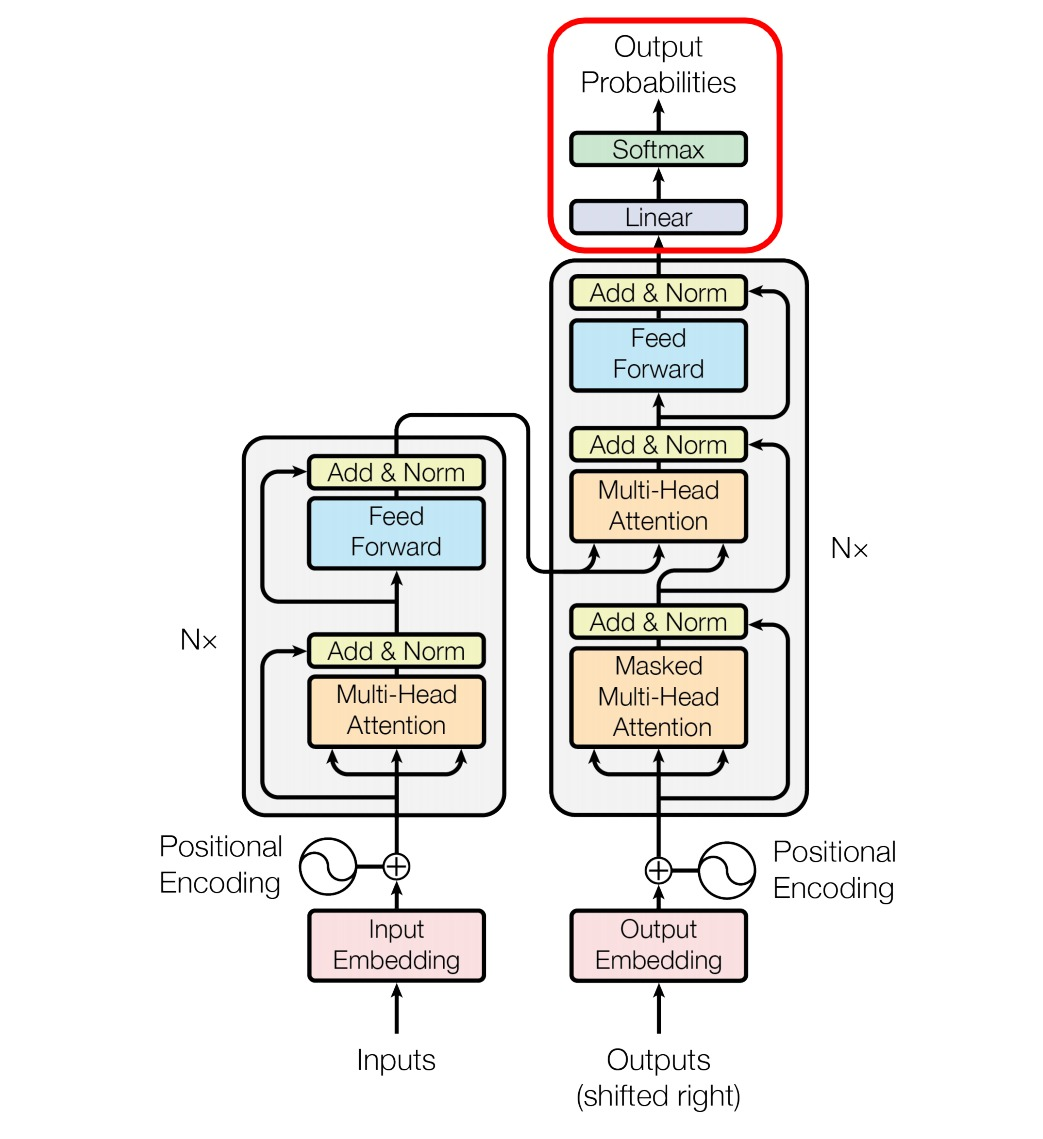
\includegraphics[height=0.9\textheight]{transformer_output}
    \raisebox{3em}{\gray{Image Adapted from \cite{vaswani_attention_2017}}}
    \pnote{
        followed by topk selection
    }
\end{frame}

\begin{frame}[c]{Parameters}
    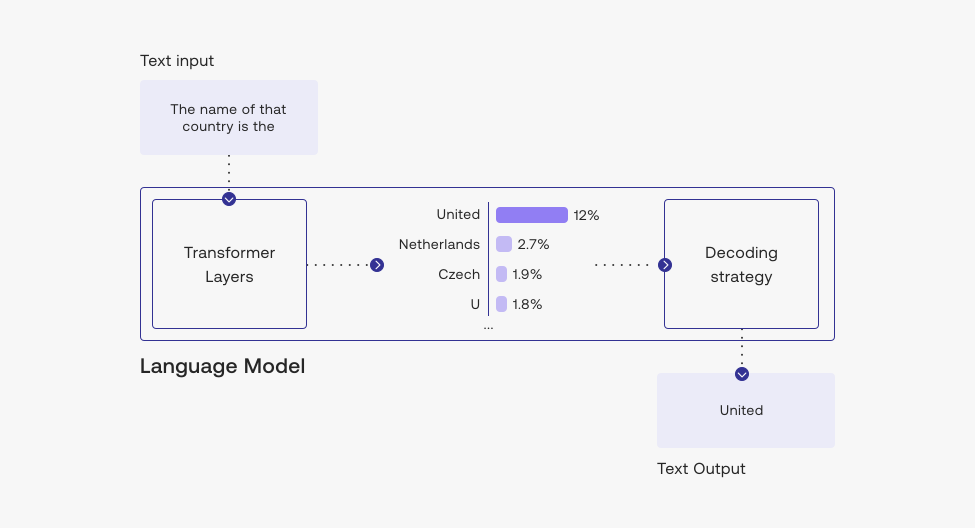
\includegraphics[width=\textwidth]{decoding_strategy} \\
    \gray{Image Source: \cite{cohereaidocs_topk_2022}}
\end{frame}


\begin{frame}[c]{Temperature, Top-k and Top-p}
    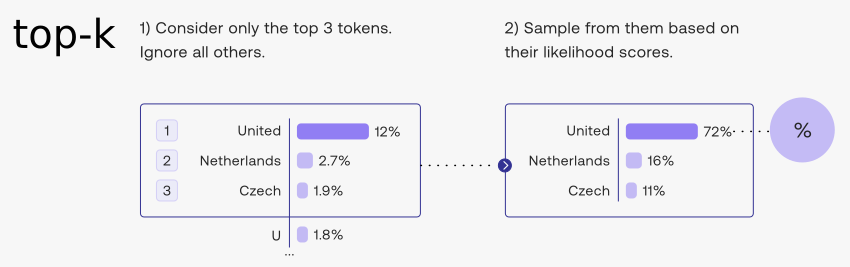
\includegraphics[width=\textwidth]{decoding_topk} \\
    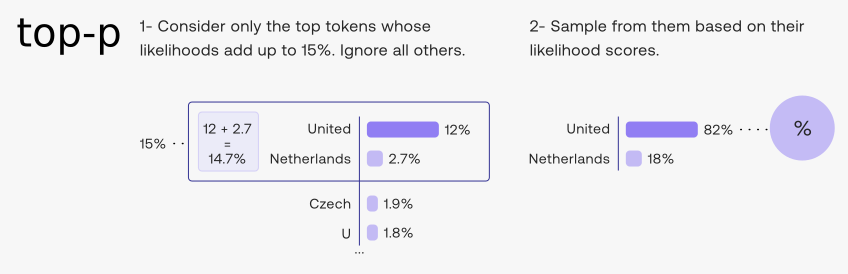
\includegraphics[width=\textwidth]{decoding_topp} \\
    \gray{Image Source: \cite{cohereaidocs_topk_2022}}
    \pnote{
        Temperature is non-linear rescaling of values, increasing chance of
        lower-likelihood predictions to be chosen.
    }
\end{frame}

\subsection{Dimensions}
\begin{frame}[c]{Dimensions at Each Step}
    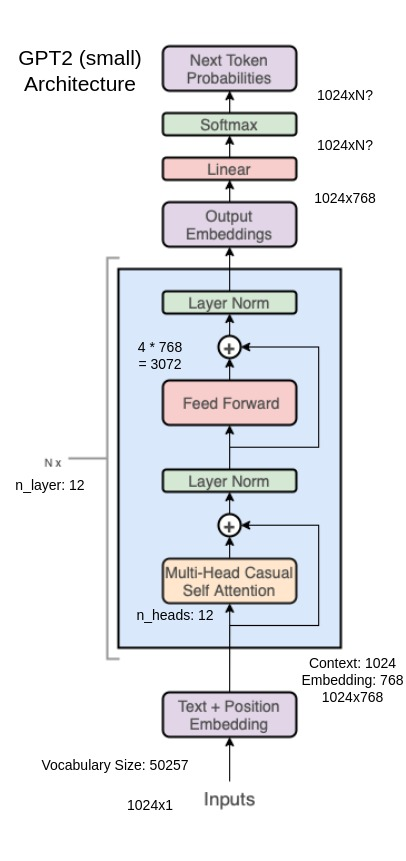
\includegraphics[height=0.9\textheight]{gpt2_decoder_dims}
    \raisebox{3em}{\gray{Image Adapted from: \cite{mody_gpt_2023}}}
    \pnote{
        Dimensions represent my current understanding
    }
\end{frame}

\begin{frame}[c]{Dimensions II}
    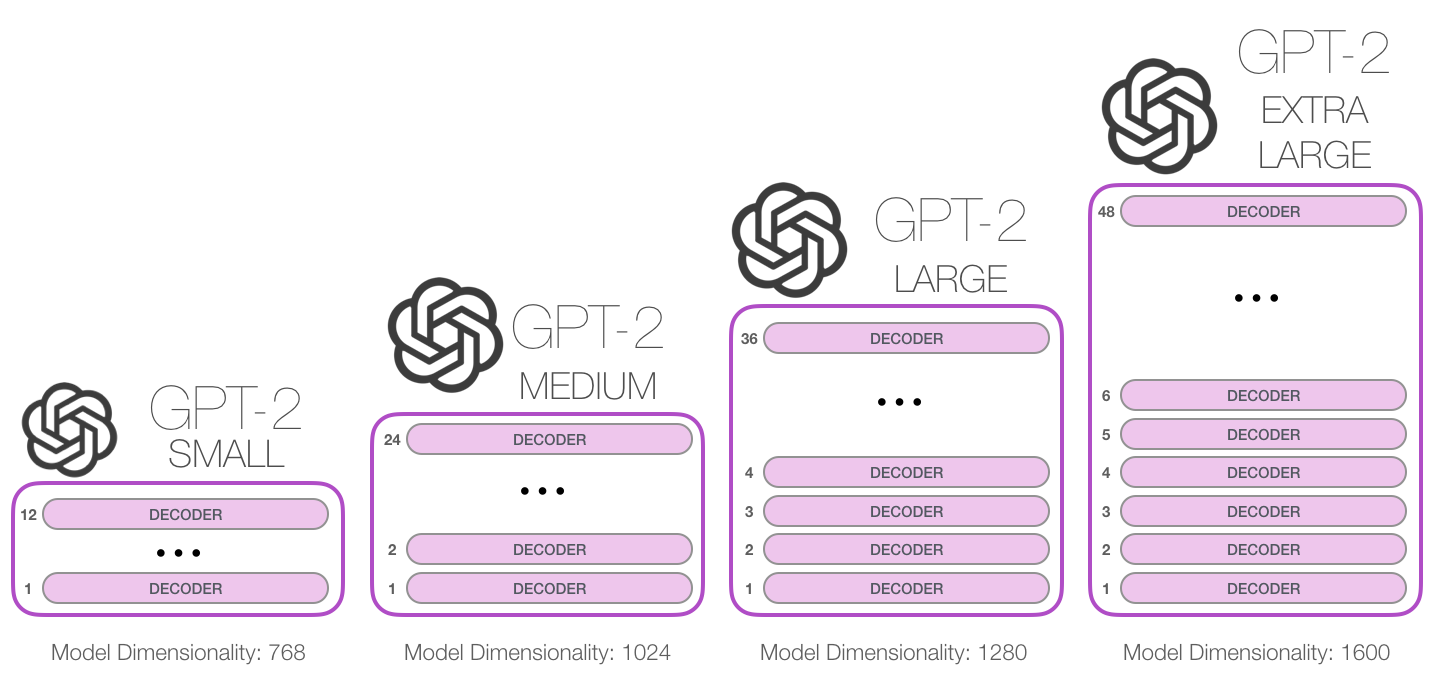
\includegraphics[width=\textwidth]{gpt2-sizes} \\
    \gray{Image Source: \cite{alammar_illustrated_2019}}
\end{frame}


\subsection{Putting it all Together}
\begin{frame}[c]{Full Architecture}
    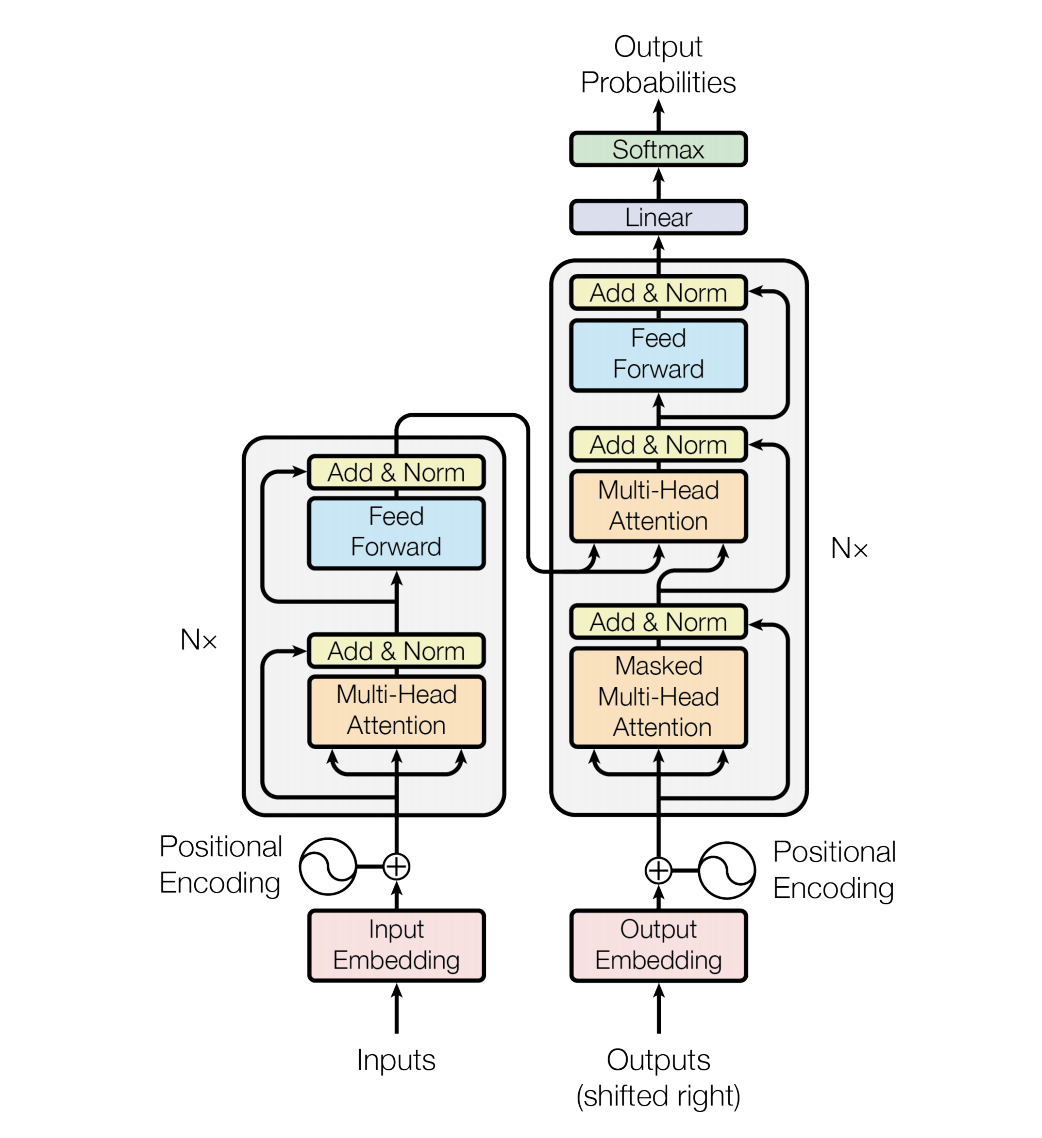
\includegraphics[height=0.9\textheight]{transformer}
    \raisebox{3em}{\gray{Image Source: \cite{vaswani_attention_2017}}}
\end{frame}

\subsection{Interpretation}
\begin{frame}[c]{One Prevalent Interpretation: Solving ODEs}
    \large
    \begin{aquote}{Lu et al., 2019 \cite{lu_understanding_2019}}
        {\em ... the Transformer can be mathematically interpreted as
        a} numerical Ordinary Differential Equation (ODE) solver for a
        convection-diffusion equation in a multi-particle dynamic
        system.
    \end{aquote}
\end{frame}


\begin{frame}[c]{A Better ODE Solver}
    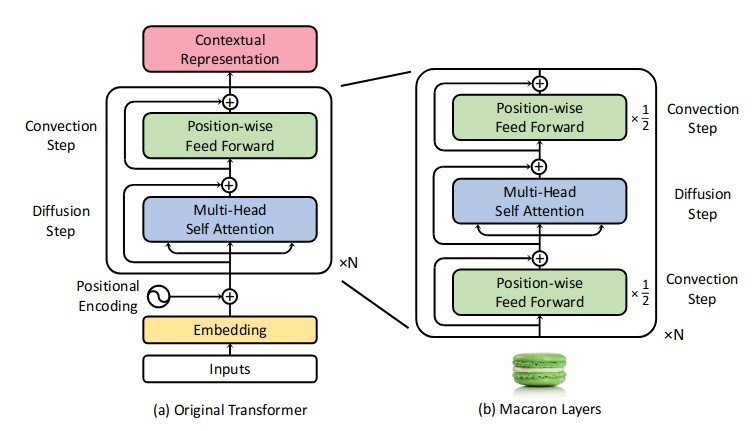
\includegraphics[width=\textwidth]{macaron_layers} \\
    \large
    For solving, use a Strang-Marchuk Splitting scheme instead of Lie-Trotter \\
    \normalsize
    \gray{Image Source: \cite{lu_understanding_2019}}
    (For details on solving methods see \cite{geiser_decomposition_2009})
    % TODO: move image source text above the additional text.
    % Doing so currently results in text overflowing of the slide, due to
    % additional space in the newline like that, for some weird reason.
    \pnote{
        they clearly showed that it could be interpreted as physical system
        with particles (tokens) interacting. For that, the solver could be
        improved. \\
        However, while they did improve results, they only did so marginally.
        I assume they didn't use it fully, more experiments necessary.
    }
\end{frame}

\begin{frame}[c]{As High-Order Nonlinearity}
    \large
    \begin{aquote}{Ye et al. 2023, Towards ... \cite{ye_understanding_2023}}
        However, we find only a weak consistency exists between the attention
        weights of features and their importance. We verify the feature map
        multiplication that brings about \textbf{high-order non-linearity into CNNs is
        crucial for the effectiveness} of attention mechanism.
    \end{aquote}
\end{frame}


\begin{frame}[c]{In-Context Optimization}
    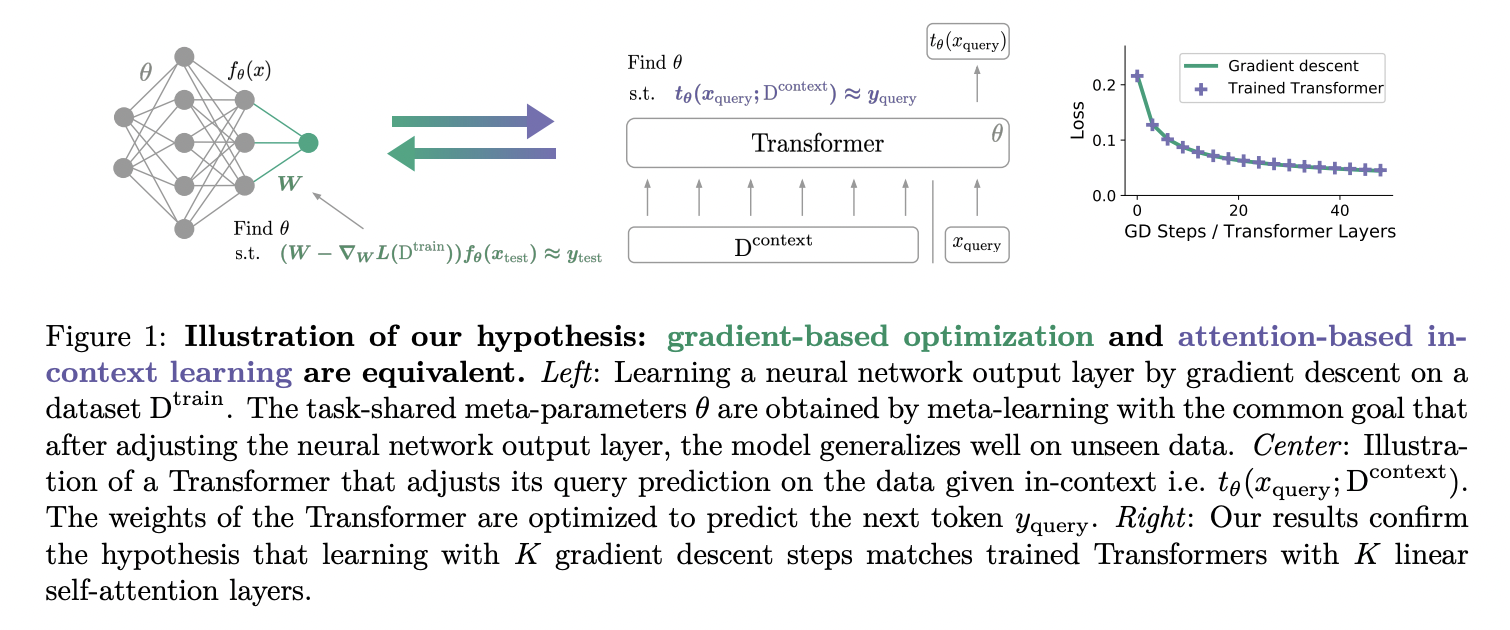
\includegraphics[width=\textwidth]{in-context} \\
    \gray{Image Source: \cite{vonoswald_transformers_2022}}
        \begin{aquote}{Transformers Learn In-Context \cite{vonoswald_transformers_2022}}
            ... training Transformers ... can be closely related to well-known
            gradient-based meta-learning formulations.
        \end{aquote}
    \pnote{
        Not sure if not actually a product of mesa-optimization \\
        \\
        information hazard note on mesa optimizers
    }
\end{frame}

\subsection{Architecture Improvements}
\begin{frame}[c]{Sparse Transformer: $O(n \sqrt{n})$ instead of $O(n^2)$}
    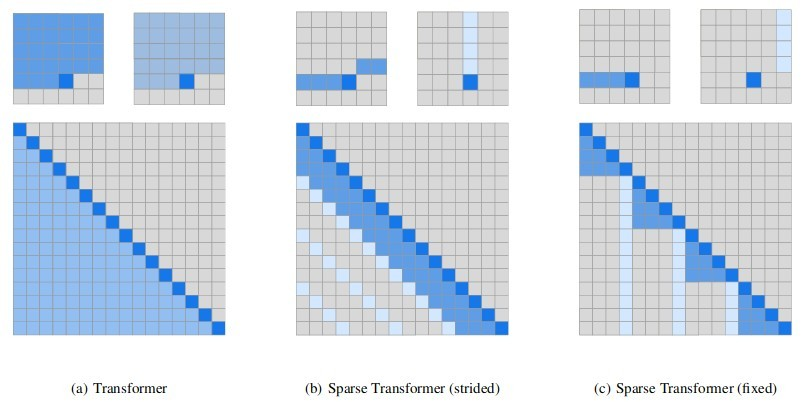
\includegraphics[width=\textwidth]{sparse_transformer} \\
    \normalsize
    \gray{Image Source: \cite{child_generating_2019}} \\
    \large
    Used first in the GPT3 family of models. \\
    A lot of other patterns are possible too
    \pnote{
    Even the original GPT didn't use 'full' transformers, but Sparse Transformer \\
    Runtime: O(n sqrt n) instead of O( n * n ) \\
    \\
    Obviously a huge benefit if you can get substantially reduced runtime \\
    for the same performance
}
\end{frame}


\begin{frame}[c]{FlashAttention}
    \large
    They realized that the bottleneck wasn't compute, but IO. \\
    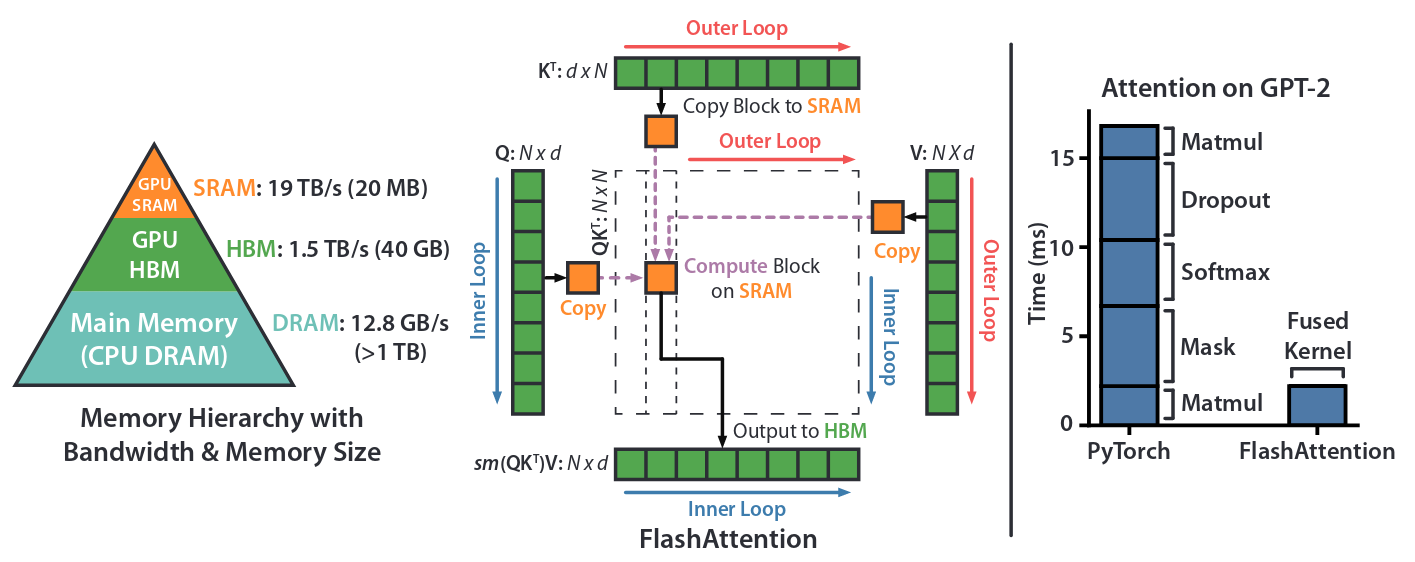
\includegraphics[width=\textwidth]{flashattention_memory} \\
    \gray{Image Source: \cite{dao_flashattention_2022}} \\
    \large
    Used first in the GPT4 family of models
    \pnote{
        From what we know, GPT4 is using a variant of FlashAttention
    }
\end{frame}


\begin{frame}[c]{FlashAttention Benchmarks}
    \large
    \begin{tabular}{c|ccc}
        Attention & Standard & FlashAttention & Ratio \\ \hline
        GFLOPs & 66.6  & 75.2 & 0.89 \\
        HBM R/W & 40.3 & 4.4 & 9.16 \\
        Runtime (ms) & 41.7 & 7.3 & 5.71 \\
    \end{tabular} \newline \newline
    \normalsize
    \gray{Table from \cite{dao_flashattention_2022}} \\
    \large
    Note that Standard Attention is $O(n^2)$ in compute.
\end{frame}

% \begin{frame}[c]{Linear-Time Transformer}
%     FastFormer \cite{wu_fastformer_2021} \\
%     Transformer Quality in Linear Time \cite{hua_transformer_2022} \\
%     \todo{linear time transformer}
% \end{frame}



\section{Compression}
\subsection{Quantization}
\begin{frame}[c]
    GPTQ \cite{frantar_gptq_2022}
    (spun up for LlaMa just two weeks after 'release')
\end{frame}

\subsection{Distillation}
\begin{frame}[c]
    Training a smaller model on outputting similar outputs distributions for given inputs
    \cite{sun_patient_2019}
    \cite{polino_model_2018}
\end{frame}

\subsection{Rank Reduction}
\begin{frame}[c]
    LoRA \cite{hu_lora_2021}
    (spun up for LlaMa just a month after 'release')
\end{frame}

\section{As Module}

\subsection{Memorizing}


\begin{frame}[c]{Memorizing Transformers}
    Memorizing Transformer \cite{wu_memorizing_2022}: kNN-augmented attention layer, can reduce parameter count 5x while keeping perplexity
\end{frame}


\begin{frame}[c]{Metrics}
    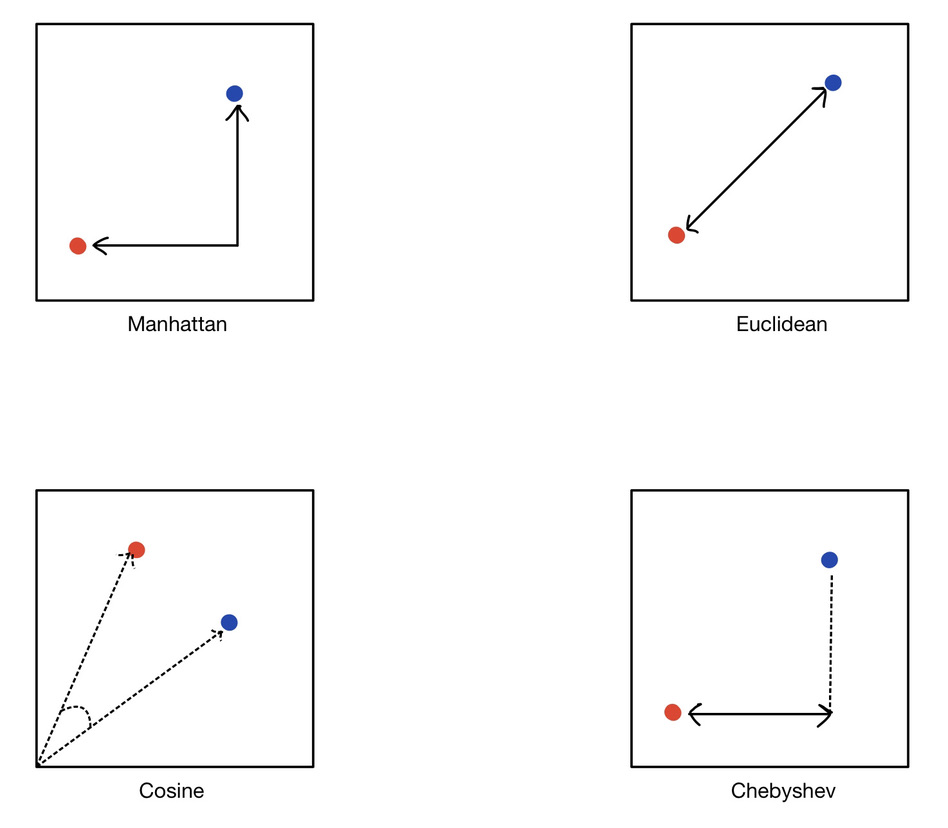
\includegraphics[width=\textwidth]{similarity-search-distance-metrics} \\
    Image Source: Public Domain
\end{frame}

\begin{frame}[c]{Vector Databases}
    Family of fast lookup vector index structures, optimized for such use cases

    Hierarchical Navigable Small Worlds (HNSW)
    \url{pinecone.io/learn/hnsw/}
\end{frame}

\section{Successes}
\subsection{BERT}
\begin{frame}[c]{BERT: Bidirectional Encoder Representations}
    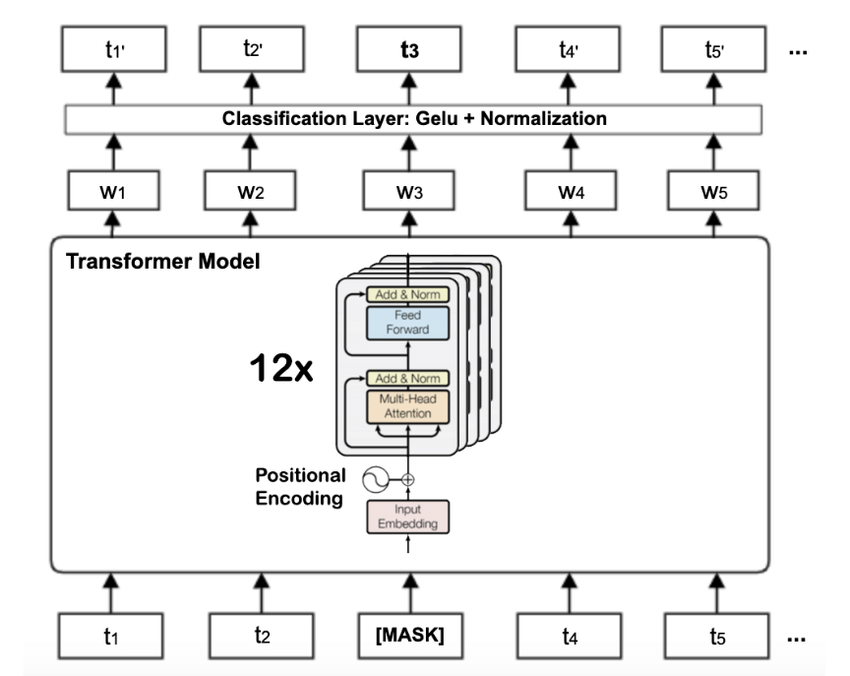
\includegraphics[height=0.8\textheight]{bert} \\
    \gray{Image Source: \cite{khalid_rubert_2021}}
    \large
    Original BERT \cite{devlin_bert_2018}
    \pnote{
        BERT is an encoder-only transformer
    }
\end{frame}

\subsection{GPT}
\begin{frame}[c]{GPT: Pure Decoder Architectures}
    \begin{columns}
        \column{0.4\textwidth}
        \begin{minipage}[c][\textheight][c]{\linewidth}
            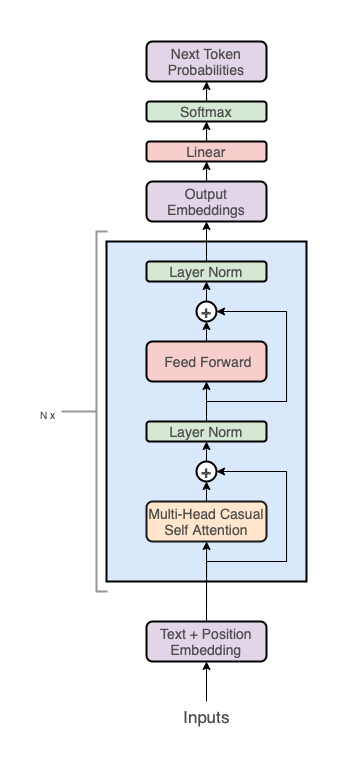
\includegraphics[height=0.8\textheight]{GPT_architecture} \\
            \gray{Image Source: \cite{mody_gpt_2023}}
        \end{minipage}
        \column{0.6\textwidth}
        \begin{minipage}[c][\textheight][c]{\linewidth}
            \large
            Examples:
            \begin{itemize}
                \item GPT \cite{radford_improving_2018}
                \item GPT2 \cite{radford_language_2019}
                \item GPT3? \cite{brown_language_2020}
                \item GPT4? \cite{openai_gpt4_2023}
                \item LlaMa \cite{touvron_llama_2023}
                \item Bloom \cite{workshop_bloom_2022}
                \item OPT \cite{zhang_opt_2022}
                \item PaLM \cite{chowdhery_palm_2022}
            \end{itemize}
        \end{minipage}
    \end{columns}
    \pnote{
        GPT3 is a question mark, but we pretty much know most about it \\
        GPT4 is a bigger question, but I have a slide for that too
    }
\end{frame}


\begin{frame}[c]{GPT4: What We Know}
    \begin{itemize}[<+(1)->]
        \item Parameters: 1.76 trillion, about 10x of GPT3
        \item Mixture of Experts (MoE) with 16 partially differently trained
            heads with 111B parameters each, asking only two for each forward
            pass
        \item Trained on 13 trillion tokens, maybe more
        \item Speculation of training costs of the final run are 63 million USD.
        \item Performance got a lot worse through lobotomization from RLHF (ChatGPT4) and using proposal networks to reduce inference costs
    \end{itemize}
    \pause
    No official source ... most of it is based on speculation from what george hotz leaked in an interview \cite{transhumanismvideos_george_2023}
    \pnote{
        Only the first two bullet points where directly from george hotz
    }
\end{frame}

\subsection{CLIP}
\begin{frame}[c]{CLIP: Multimodal Embedding Spaces}
    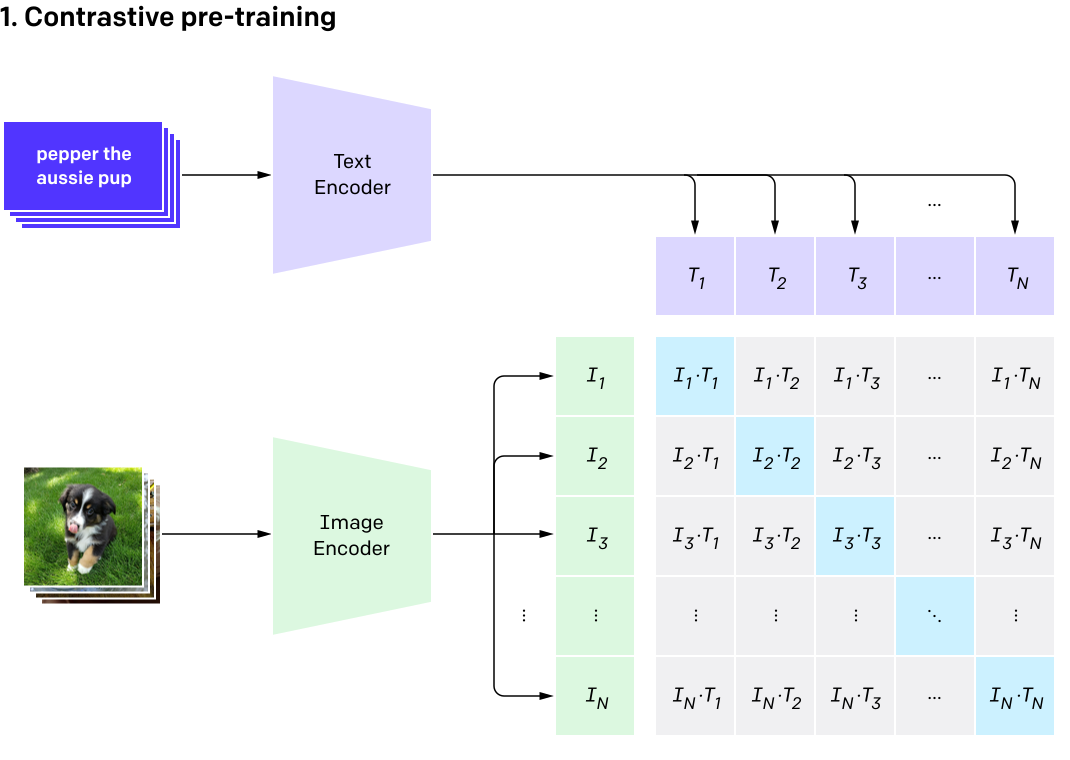
\includegraphics[height=0.8\textheight]{clip} \\
    \gray{Image Source: \cite{radford_learning_2021}}
    \large We can now describe images!
    \pnote{
        we now have an shared embedding between text and images \\
        \\
        Specifically we can determine \\
        how well a description matches an image
    }
\end{frame}

\subsection{Latent Diffusion Models}
\begin{frame}[c]{Latent Diffusion Models}
    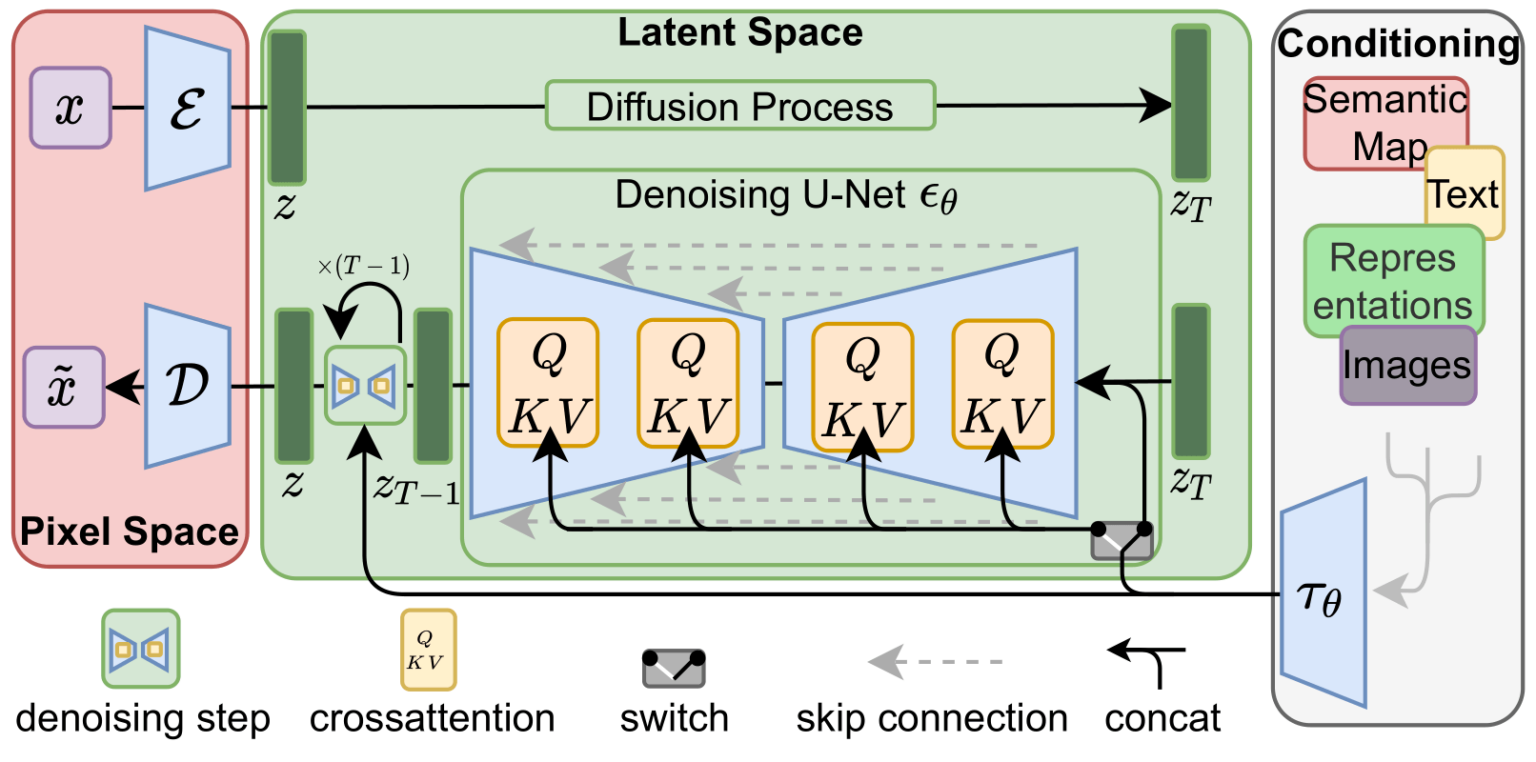
\includegraphics[width=\textwidth]{stable_diffusion} \\
    \gray{Image Source: \cite{rombach_highresolution_2022}}
    \large We can now generate images! \\
    \normalsize
    (We can also do that using GANs \cite{esser_taming_2021})
    % Generating images based on shared semantic embeddings
    % Diffusion \cite{sohl-dickstein_deep_2015}
\end{frame}

\subsection{Reinforcement Learning}
\begin{frame}[c]{GATO: A Generalist Agent}
    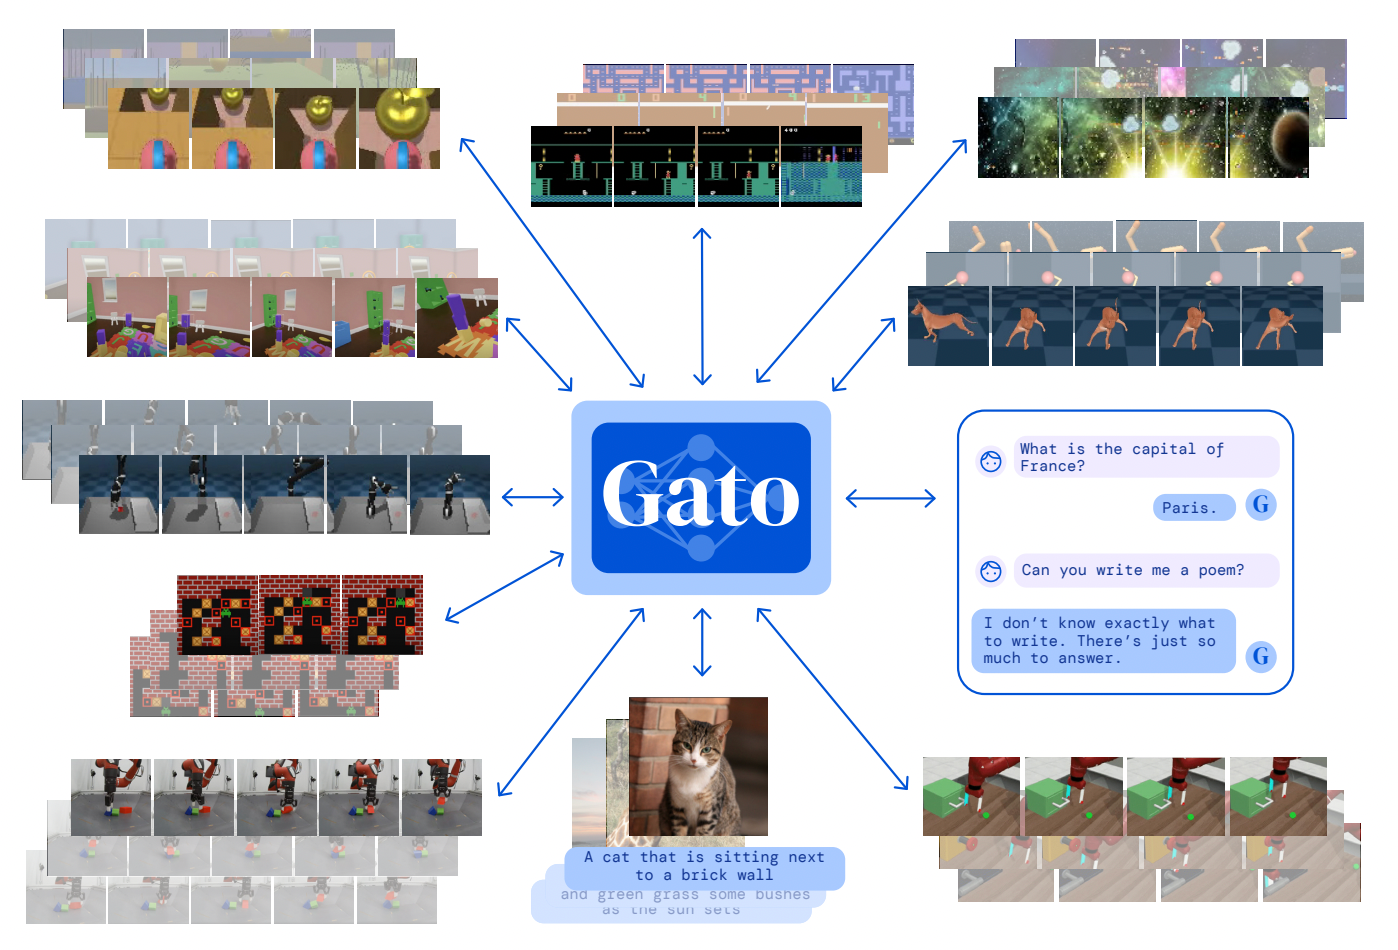
\includegraphics[height=0.8\textheight]{gato} \\
    \gray{Image Source: \cite{reed_generalist_2022}}
    \pnote{
        And more recently something something model-based RL
    }
\end{frame}

\subsection{Physics Simulation}
\begin{frame}[c]{Physics Simulation in Latent Spaces}
    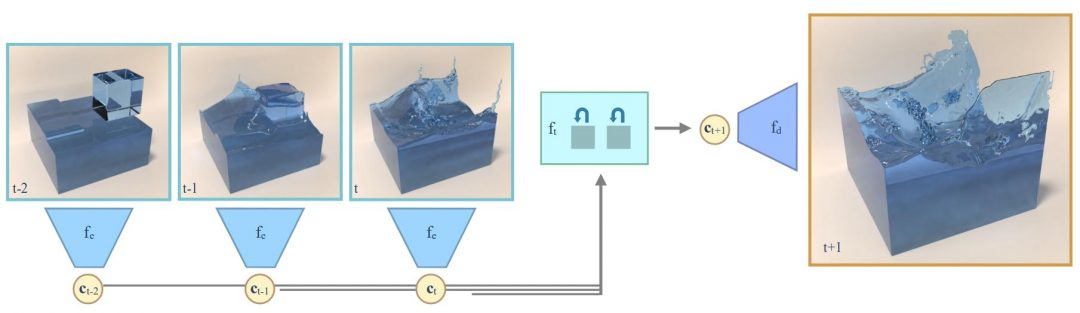
\includegraphics[height=0.8\textheight,width=\textwidth,keepaspectratio]{lsp} \\
    \gray{Image Source: \cite{wiewel_latent_2019}}
    \large
    \begin{aquote}{Latent Space Physics \cite{wiewel_latent_2019}}
        ... we arrive at a data-driven solver that yields practical speed-ups, and
        at its core is more than 150x faster than a regular pressure solver.
    \end{aquote}
    \pnote{
        Speed up simulation by 150x 
    }
\end{frame}

\subsection{Capability}

\begin{frame}[c]{Current Progress is Exponential}
    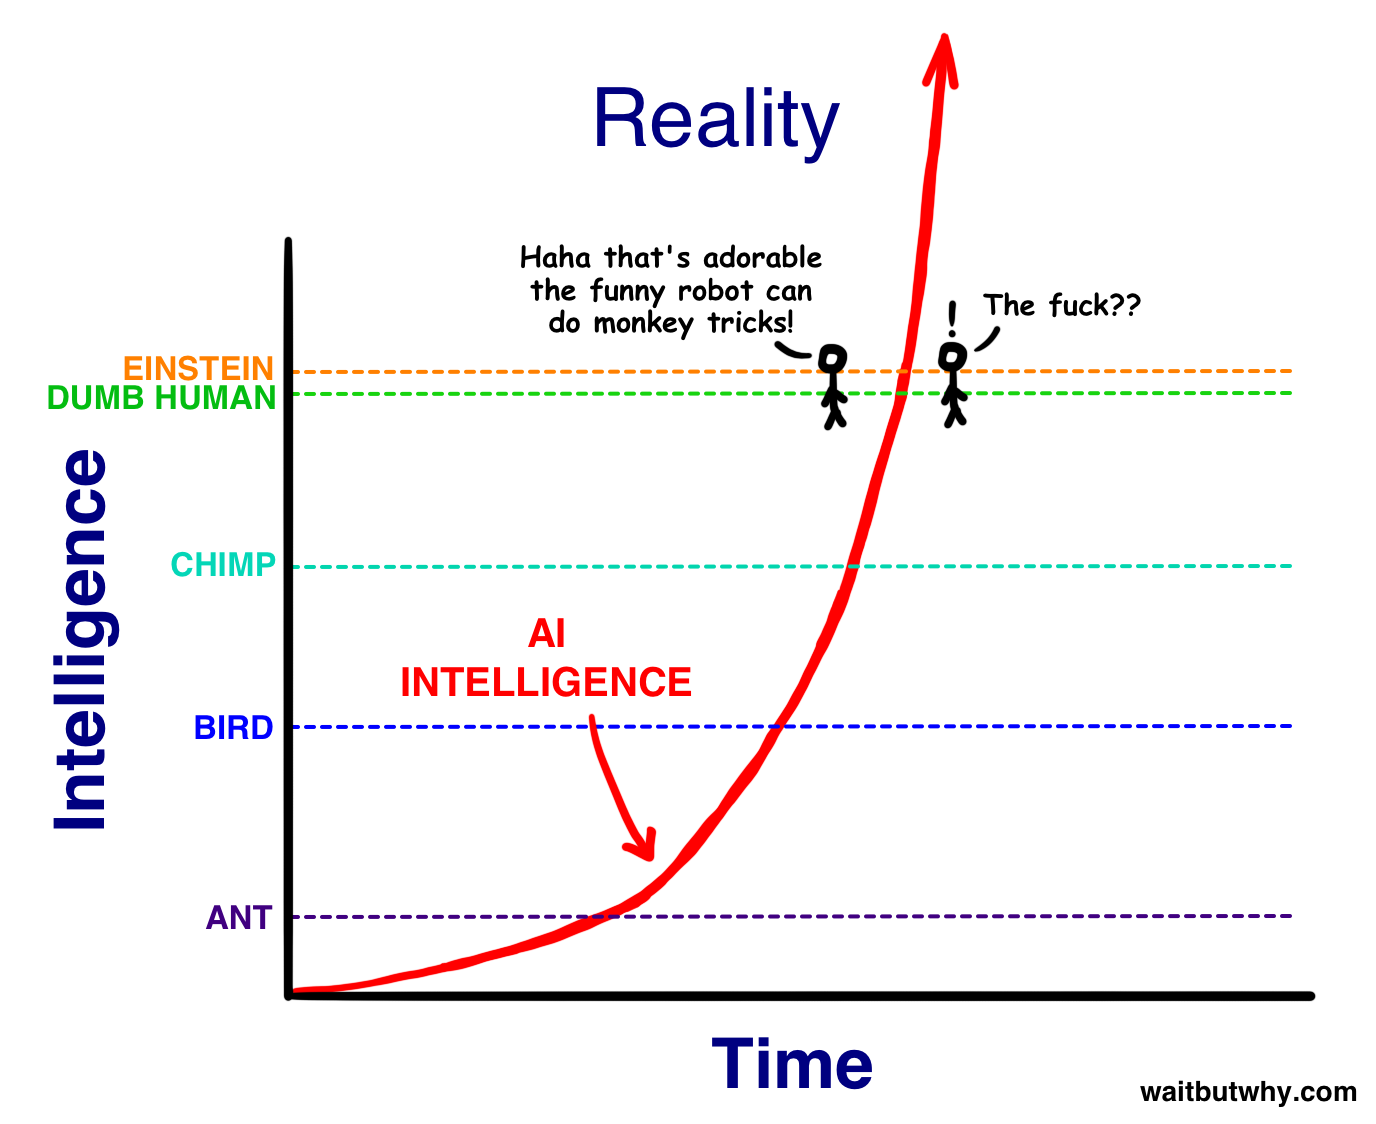
\includegraphics[height=0.8\textheight]{Intelligence2} \\
    \gray{Image Source: \cite{urban_artificial_2015}}
\end{frame}

% \subsection{Meta Cognition}
% \begin{frame}[c]{Reflexion}
%     Reflexion \cite{shinn_reflexion_2023}
%     \todo{include architecture}
% \end{frame}

% \begin{frame}[c]{Architecture Changes}
%     \begin{itemize}[<+(1)->]
%         \item No Encoder part, GPTs are autoregressive decoder-only
%         \item LayerNorm before, not after Layers
%         \item Positional Encoding for each intermittent Layer 
%     \end{itemize}
% \end{frame}

\section{Limitations}

\begin{frame}[c]{Limitations} 
    \large
    \begin{itemize}[<+(1)->]
        \item Hallucination: Output could be plain wrong
        \item Spatial Reasoning: Difficult from text alone
        \item Planning beyond the next step
    \end{itemize}
    A list of failures: \cite{borji_categorical_2023}
\end{frame}

% \subsection{Hallucination}
% \begin{frame}[c]{Hallucination}
%     Just plain wrong
% \end{frame}
% 
% \subsection{Spatial Reasoning}
% \begin{frame}[c]
%     GPT3 issues
% \end{frame}
% 
% \subsection{Forward-Planning}
% \begin{frame}[c]
%     Asked to answer in exactly $<n>$ words
% \end{frame}
% 


\section{Conclusion}


\begin{frame}[c]{Review}
    We made substantial Progress!
\end{frame}

\begin{frame}[c]{Next Steps}
    There's a bunch of stuff still left to do:
    \begin{itemize}[<+(1)->]
        \item Deployment of the newly implemented features
        \item Adapt design to current KIT corporate design
        \item Finish dynamic \mintinline{python}{PersonForms} implementation
        \item Login with non-unique identifiers (EPPN)
        \item Advanced User Administration of Accounts
        \item Realizing Projects through Storage API-Access
        \item ...
    \end{itemize}
\end{frame}




% '\include'
% - gives speed bonus when building, through caching in a seperate *.aux file
% - has a 'page break'
% - cannot be nested
% ------------- VS -------------
% '\input'
% - can be nested
% - does not have 'page breaks'
% - gives no caching benefit


%%%%%%%%%%%%%%%%%%%%%%%%%%%%%%%%%%%%%%%%%%%%%%%%%%%%%%%%%%%%%%%%%%%%%%%%%%%%%%%%%%%%%%%%%%%%%%%%%%%



%%%%%%%%%%%%%%%%%%%%%%%%%%%%%%%%%%%%%%%%%%%%%%%%%%SOURCES%%%%%%%%%%%%%%%%%%%%%%%%%%%%%%%%%%%%%%%%%%

\begin{frame}[c,fragile,allowframebreaks]{Sources}
% \bibliographystyle{plainnat}
\bibliographystyle{ieeetr}
\bibliography{references.bib}
\end{frame}


\addtocounter{framenumber}{1}
\begin{frame}[standout]
    \Huge
    End
\end{frame}

\appendix
\backupbegin

\section{Statistics}


\begin{frame}[c]{LOC by Author}
    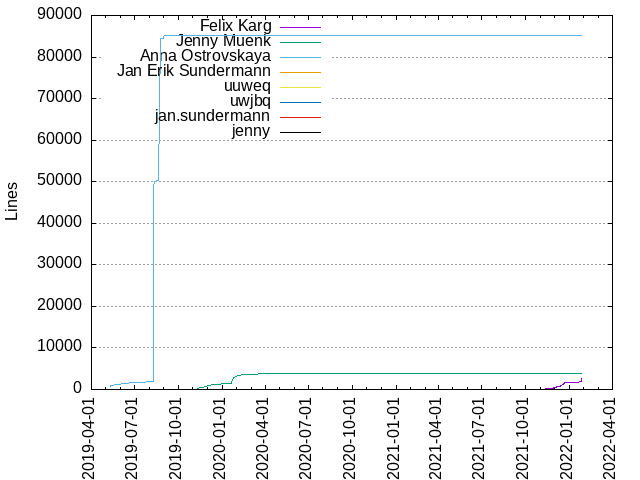
\includegraphics[height=\textheight]{lines_of_code_by_author}
\end{frame}

\begin{frame}[c]{Commits by Author}
    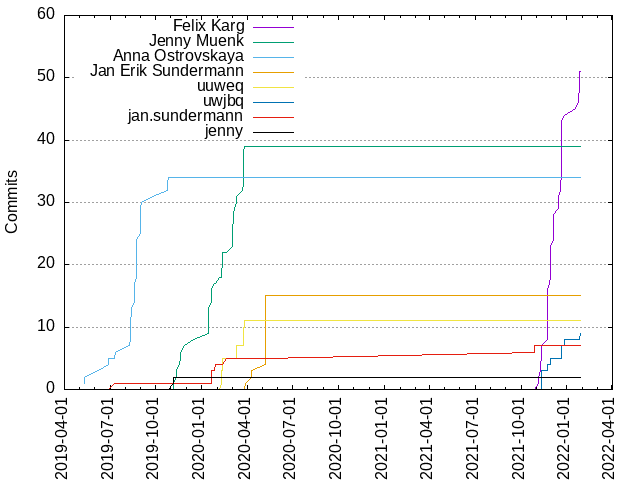
\includegraphics[height=\textheight]{commits_by_author}
\end{frame}

\pic{Recent Activity (Commits by Week)}{34}


\begin{frame}[c,fragile]{LOC stats: Before}
    \large
    \begin{tabular}{l:r:r:r:r:r}
        Language & Files & Lines & Code & Comments & Blanks \\ \hline
CSS           &        28 &      19144 &      17235 &        284 &       1625 \\
JavaScript    &        27 &      63499 &      43096 &      13725 &       6678 \\ \hdashline
Python        &        34 &       1812 &       1510 &         56 &        246 \\
SVG           &        14 &         14 &         14 &          0 &          0 \\ \hdashline
HTML          &        10 &        938 &        838 &         30 &         70 \\
|- CSS        &         1 &        312 &        282 &         28 &          2 \\
|- JavaScript &         5 &        155 &        126 &         13 &         16 \\ \hdashline
Total         &       122 &      86008 &      62693 &      14627 &       8688 \\
    \end{tabular} \\
    \scriptsize \newline (The numbers don't quite add up, because I omitted e.g. Configs, Markdown, ...)
\end{frame}

\begin{frame}[c,fragile]{LOC stats: After}
    \large
    \begin{tabular}{l:r:r:r:r:r}
        Language & Files & Lines & Code & Comments & Blanks \\ \hline
        CSS            &       28   &    19162    &   17248   &      284    &    1630 \\
        JavaScript     &       27   &    63499    &   43096   &    13725    &    6678 \\ \hdashline
        Python         &       48   &     3078    &    2485   &      160    &     434 \\
        SVG            &       14   &       14    &      14   &        0    &       0 \\ \hdashline
        HTML           &       15   &     1231    &    1107   &       39    &      85 \\
        |- CSS         &        1   &      312    &     282   &       28    &       2 \\
        |- JavaScript  &        7   &      244    &     202   &       21    &      21 \\ \hdashline
        Total          &      134   &    87055    &   63960   &    14245    &    8850 \\
    \end{tabular} \\
    \scriptsize \newline (The numbers don't quite add up, because I omitted e.g. Configs, Markdown, ...)
\end{frame}


\begin{frame}[c,fragile]{LOC stats: Diff}
    \large
    \begin{tabular}{l:r:r:r:r:r}
        Language & Files & Lines & Code & Comments & Blanks \\ \hline
        CSS            &        0   &    \p{18}   &   \p{13}  &        0    &    \p{5} \\
        JavaScript     &        0   &        0    &       0   &        0    &       0  \\ \hdashline
        Python         &    \p{14}  &  \p{1266}   &  \p{975}  &   \p{104}   &  \p{188} \\
        SVG            &        0   &        0    &       0   &        0    &       0  \\ \hdashline
        HTML           &     \p{5}  &   \p{293}   &  \p{269}  &     \p{9}   &   \p{15} \\
        |- CSS         &        0   &        0    &       0   &        0    &       0  \\
        |- JavaScript  &     \p{2}  &    \p{89}   &   \p{76}  &     \p{8}   &    \p{5} \\ \hdashline
        Total          &    \p{12}  &  \p{1047}   & \p{1267}  &   \p{382}   &  \p{162} \\
    \end{tabular} \\
    \scriptsize \newline (The numbers don't quite add up, because I omitted e.g. Configs, Markdown, ...)
\end{frame}

\section{More Screenshots}
\subsection{Project Approval}
\pic{Project Pending}{14}
\pic{State Change Message}{15}
\pic{Project Approved}{17}
\pic{State Change Message}{16}

\subsection{Requesting More Storage}
\pic{Extension Requests: The Project Needs to be Approved}{18}
\pic{Timeframe Extension Request View}{19}
% \pic{lsdf.kit.edu/extension/timeframe/9/create/}{19}
\pic{Capacity Extension Request View}{20}
\pic{Filled out Capacity Extension}{21}
\pic{Extension System Message}{22}

\begin{frame}[c]{Projects Admin View}
                           % trim=left bottom right top, clip
    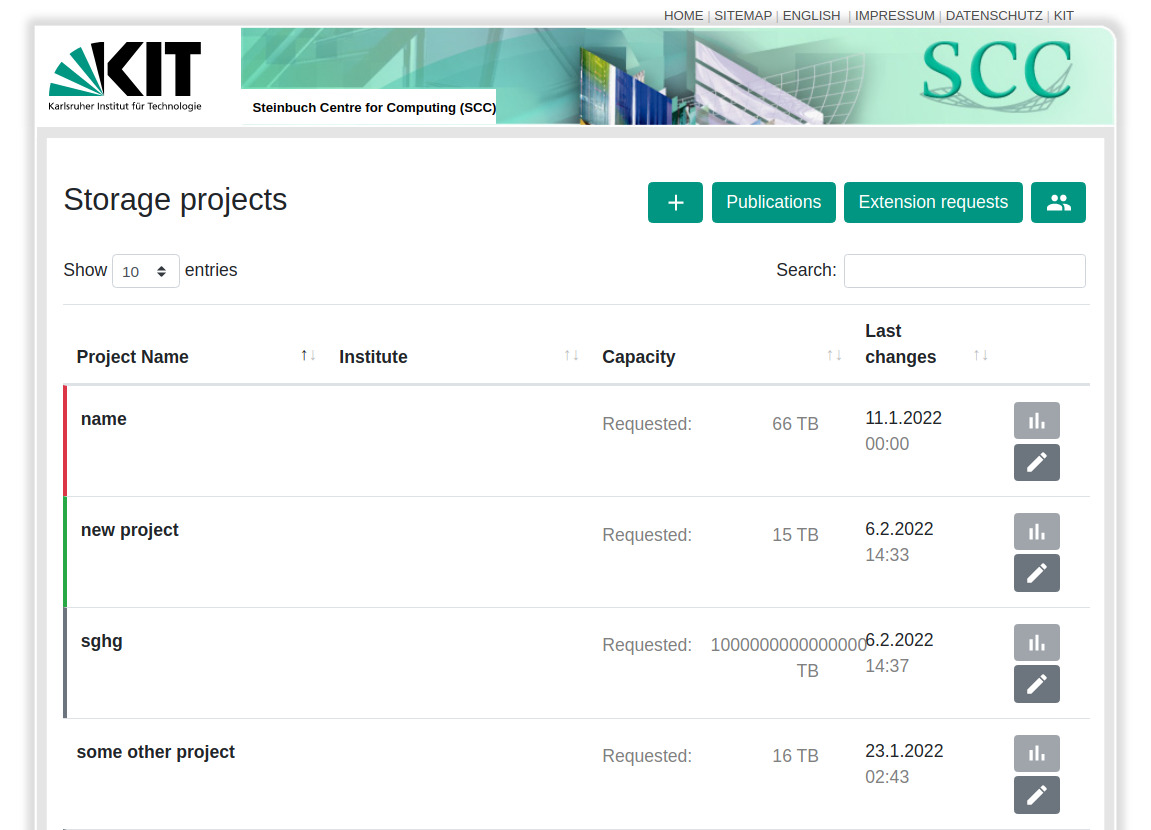
\includegraphics[width=\textwidth,trim=0 0 0 150,clip]{Selection_023}
\end{frame}

% 24 and 25 don't exist
\pic{Extension Request Overview}{26}
\pic{Approving Request}{27}
\pic{System Message showing Extension Approval}{28}
\pic{Increased Capacity from User View}{29}


\backupend


\end{document}
